%*****************************************************A**************************
%********************************** Chapter XXXXXXXX ***************************
%*******************************************************************************

\newcommand{\BigO}[1]{\ensuremath{\operatorname{O}\bigl(#1\bigr)}}

\nomenclature[z-MIP]{MIP}{Minimum Ionising Particle}
\nomenclature[z-MPV]{MPV}{Most Probable Value} 
\nomenclature[z-PID]{PID}{Particle IDentification}
\nomenclature[z-PID]{PID}{Particle IDentification A}
\nomenclature[z-ROI]{ROI}{Region Of Interest}

\chapter{Simulations of the 35 ton prototype} \label{chap:35tonSim} %Title of chapter

\graphicspath{ {35tonSimulation/Figs/Raster/} {35tonSimulation/Figs/PDF/} {35tonSimulation/Figs/Vector/} }

%********************************** %First Section  *************************************
\section{Determination of interaction times} \label{sec:SimInteractionTimes} %Section - X.1
As outlined at the end of Section~\ref{sec:LArSoft}, it is important to know the interaction time of a track when performing reconstruction. When performing simulations, the simplest interaction time to assign to a reconstructed object is the Monte Carlo truth time of when the particle was created. The generation time can be used, as the time taken to travel the distances considered in simulations (less than 100 ns), is small when compared to the resolution of the detector (500 ns). When matching a reconstructed object with a GEANT4 particle, the particle which contributed the most overall deposited charge to the whole track is chosen. In order to calculate this, the energy contribution of each particle to the total energy for each hit on the track is calculated. The particle which contributed the most overall charge to the track is then calculated by the summing the energy contributions for all particles, over all hits in the track. The ability to calculate the true interaction times of 3D objects, such as tracks, is vital when wanting to benchmark how well other algorithms estimate interaction times, or to determine the efficiency of the tracking algorithms, as described in Section~\ref{sec:SimRecoEffic}. \\

It was envisioned that there would be at least two ways in which interaction times could be assigned to tracks in the 35 ton detector, one using the external cosmic ray counters, and another using reconstructed scintillation light collected by the photon detectors. The cosmic ray counters were used extensively in the 35 ton data, as described in Section~\ref{sec:DataAlgs}. However, in simulations the scintillation light was used, as this would have been more powerful during continuous running. This is because not all particles entering the detector would pass through the counters, but one would expect almost all of them to produce reconstructable scintillation light. The flashes of light are reconstructed using a pre-built library, which models the expected number of photoelectrons that would be measured on each photon detector, given the 3D position of the source of the flash. Using this library, it is then possible to reconstruct the location of a flash in three dimensions, given the relative amounts of light that each photon detector collects. For example, less scintillation light will be collected for a flash that originated further away from the photon detectors. This library also takes into account the expected quantum efficiencies of each photon detector. \\

When trying to produce an association metric, a sample of 10,000 isolated positive muons generated with CRY at $T$ = 0 is used. Isolated positive muons are used, as then the events should only contain one muon track, and one reconstructed flash. This should mean that matching the track and flash is trivial. The positive muons are generated outside of the detector with a constant $y$ position, above the uppermost scintillation counters, and flat distributions in $x$ and $z$. It was clear that the photon detector reconstruction in the simulations worked well, when using the pre-built libraries, as the reconstructed flash source normally lay very close to the track which caused it. It was found that a Point of Closest Approach (PoCA) calculation, between points on the reconstructed track, and the reconstructed flash centre, gave an effective metric by which the flash and track could be associated. Other metrics, such as the distance between the flash and track centres, and the perpendicular distance between the flash centre, and the line joining the start and end of track were investigated, but found to provide less reliable metrics. The latter of these metrics is less effective because the reconstructed tracks are rarely straight lines, due to particles scattering as they travel through the LAr. Therefore, calculating the separation between the track and the flash for each point along the track, will result in a smaller minimum separation being calculated. A comparison of these metrics is shown in Figure~\ref{fig:PDYZDist}. \\

\begin{figure}
  \centering
  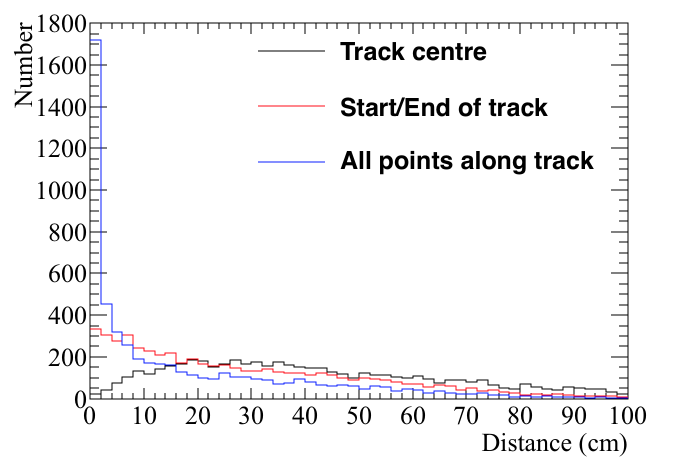
\includegraphics[width=0.6\textwidth]{DiffTrackSeps}
  \caption[Matching tracks and flashes in the 35 ton using positions in the $yz$ plane]
          {The number of events as a function of the calculated distance between a reconstructed track, and a reconstructed flash, for various metrics. Black: the distance between the track centre and the flash centre. Red: the perpendicular distance between the flash centre, and the line joining the start and end of the track. Blue: the point of closest approach between the flash centre, and all hits along the track.}
  \label{fig:PDYZDist}
\end{figure}

Another metric by which flashes could be assigned to reconstructed tracks, is by utilising the relationship between the number of measured photoelectrons in the simulation, and the distance from the APAs at which they were produced. When considering two flashes of scintillation light that are produced at different distances from the APAs, it would be expected that more photoelectrons would be collected when the photons were produced closer to the APAs. This relationship is shown in Figure~\ref{fig:NumPE_Distance}, where it can be seen that as drift distance increases, the number of measured photoelectrons decays exponentially. This relationship means that the distance between the APAs and the source of the flash, can be predicted from the number of measured photoelectrons. The predicted separation of the flash source and the APAs, can then be compared to the expected $x$ position of a reconstructed track, given the difference in flash time and hit times (Figure~\ref{fig:PD_PEDiffX}). The difference in these two quantities can then be used as a second metric, as it gives a measure of how well matched the reconstructed flash and track are. The number of flash/track combinations which are ``well matched,'' can be seen by the collection of points around the $y=x$ line in Figure~\ref{fig:PD_PEDiffX}. These points correspond to flash/track combinations where the predicted and reconstructed $x$ positions are identical, and so the metric has very accurately predicted the interaction time of the flash. \\

\begin{figure}
  \centering
  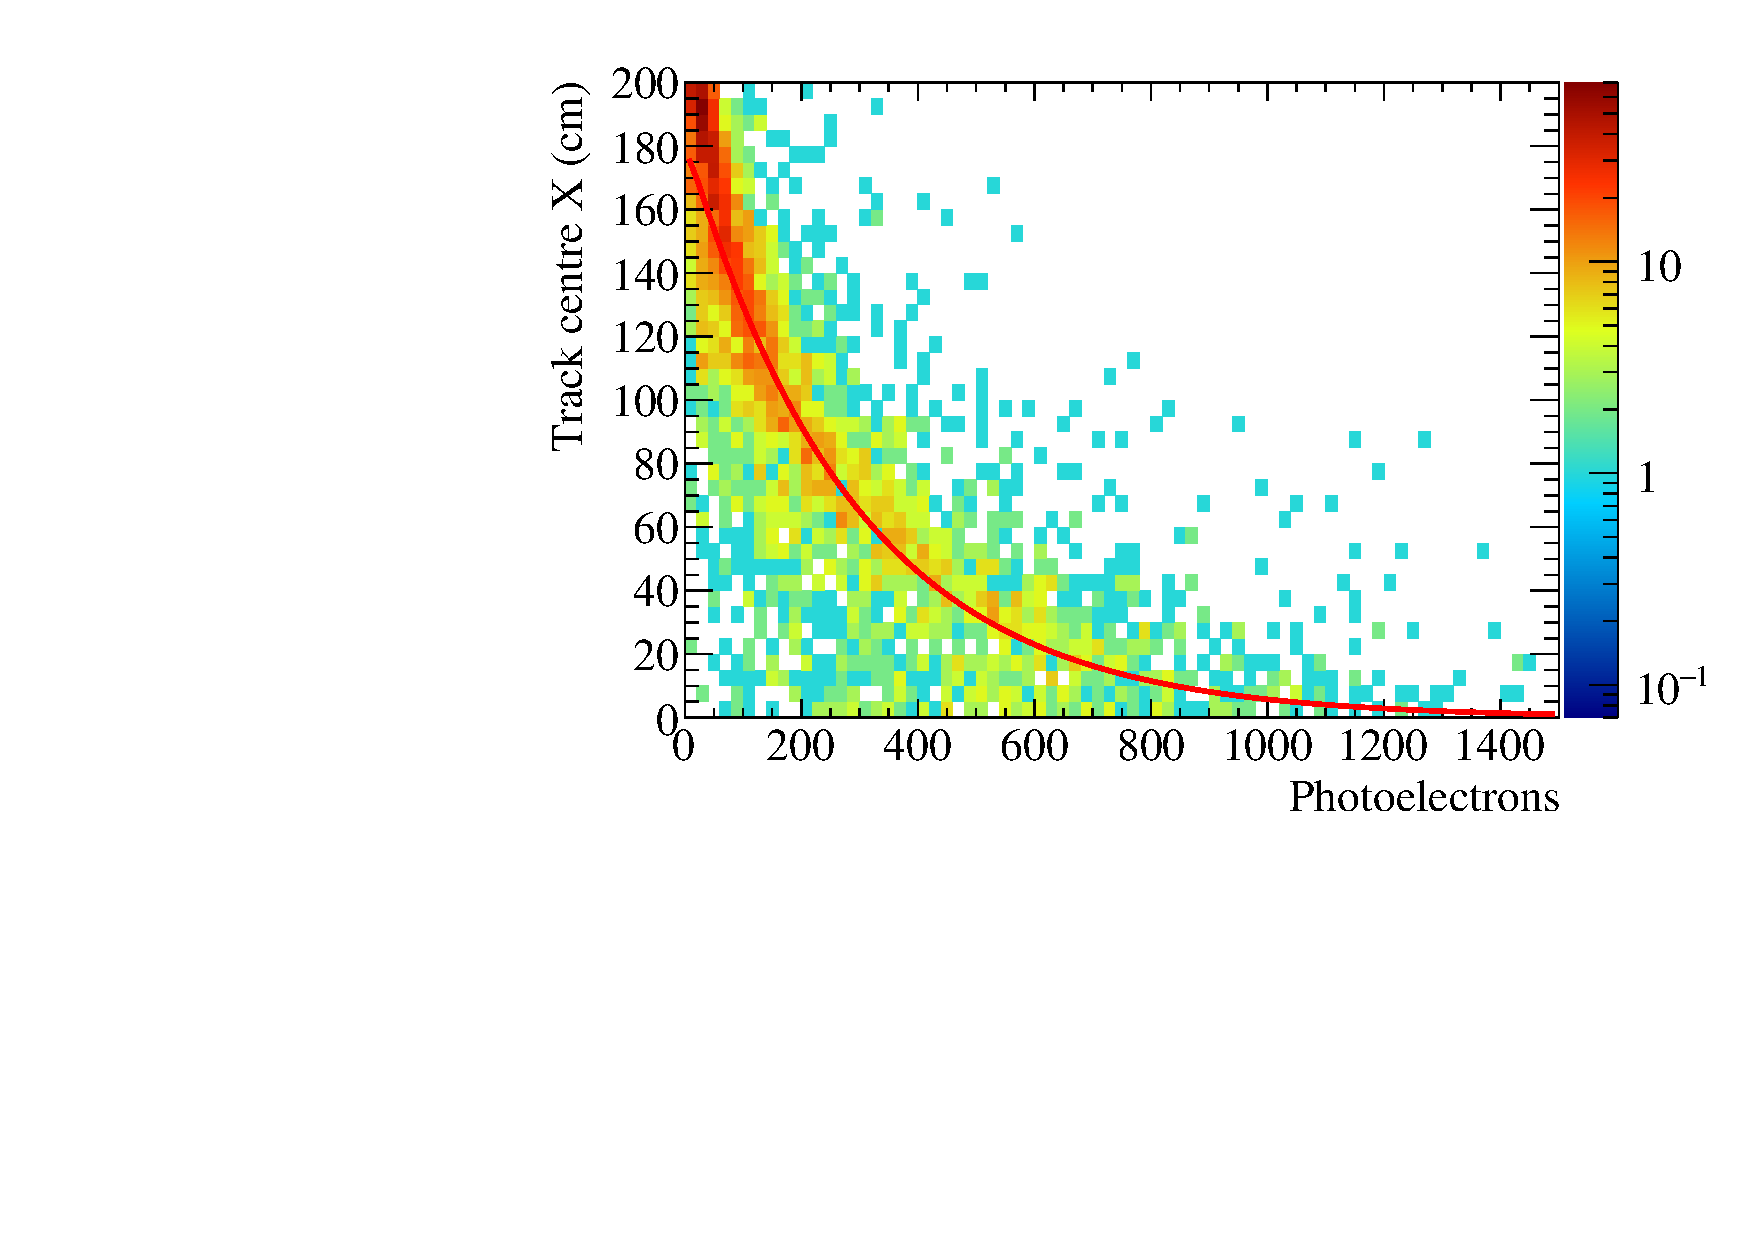
\includegraphics[width=0.6\textwidth]{NumPE_Distance}
  \caption[The central $x$ position of a reconstructed track versus the number of detected photoelectrons]
          {The central $x$ position of a reconstructed track versus the number of detected photoelectrons. The red line corresponds to a parameterisation of the distribution, which is used to predict the distance between the APAs and the flash source, given the number of measured photoelectrons in the flash. Using this parameterisation, the flash can be matched with a reconstructed track, whose centre is the same distance from the APAs.}
  \label{fig:NumPE_Distance}
\end{figure}

\begin{figure}
  \centering
  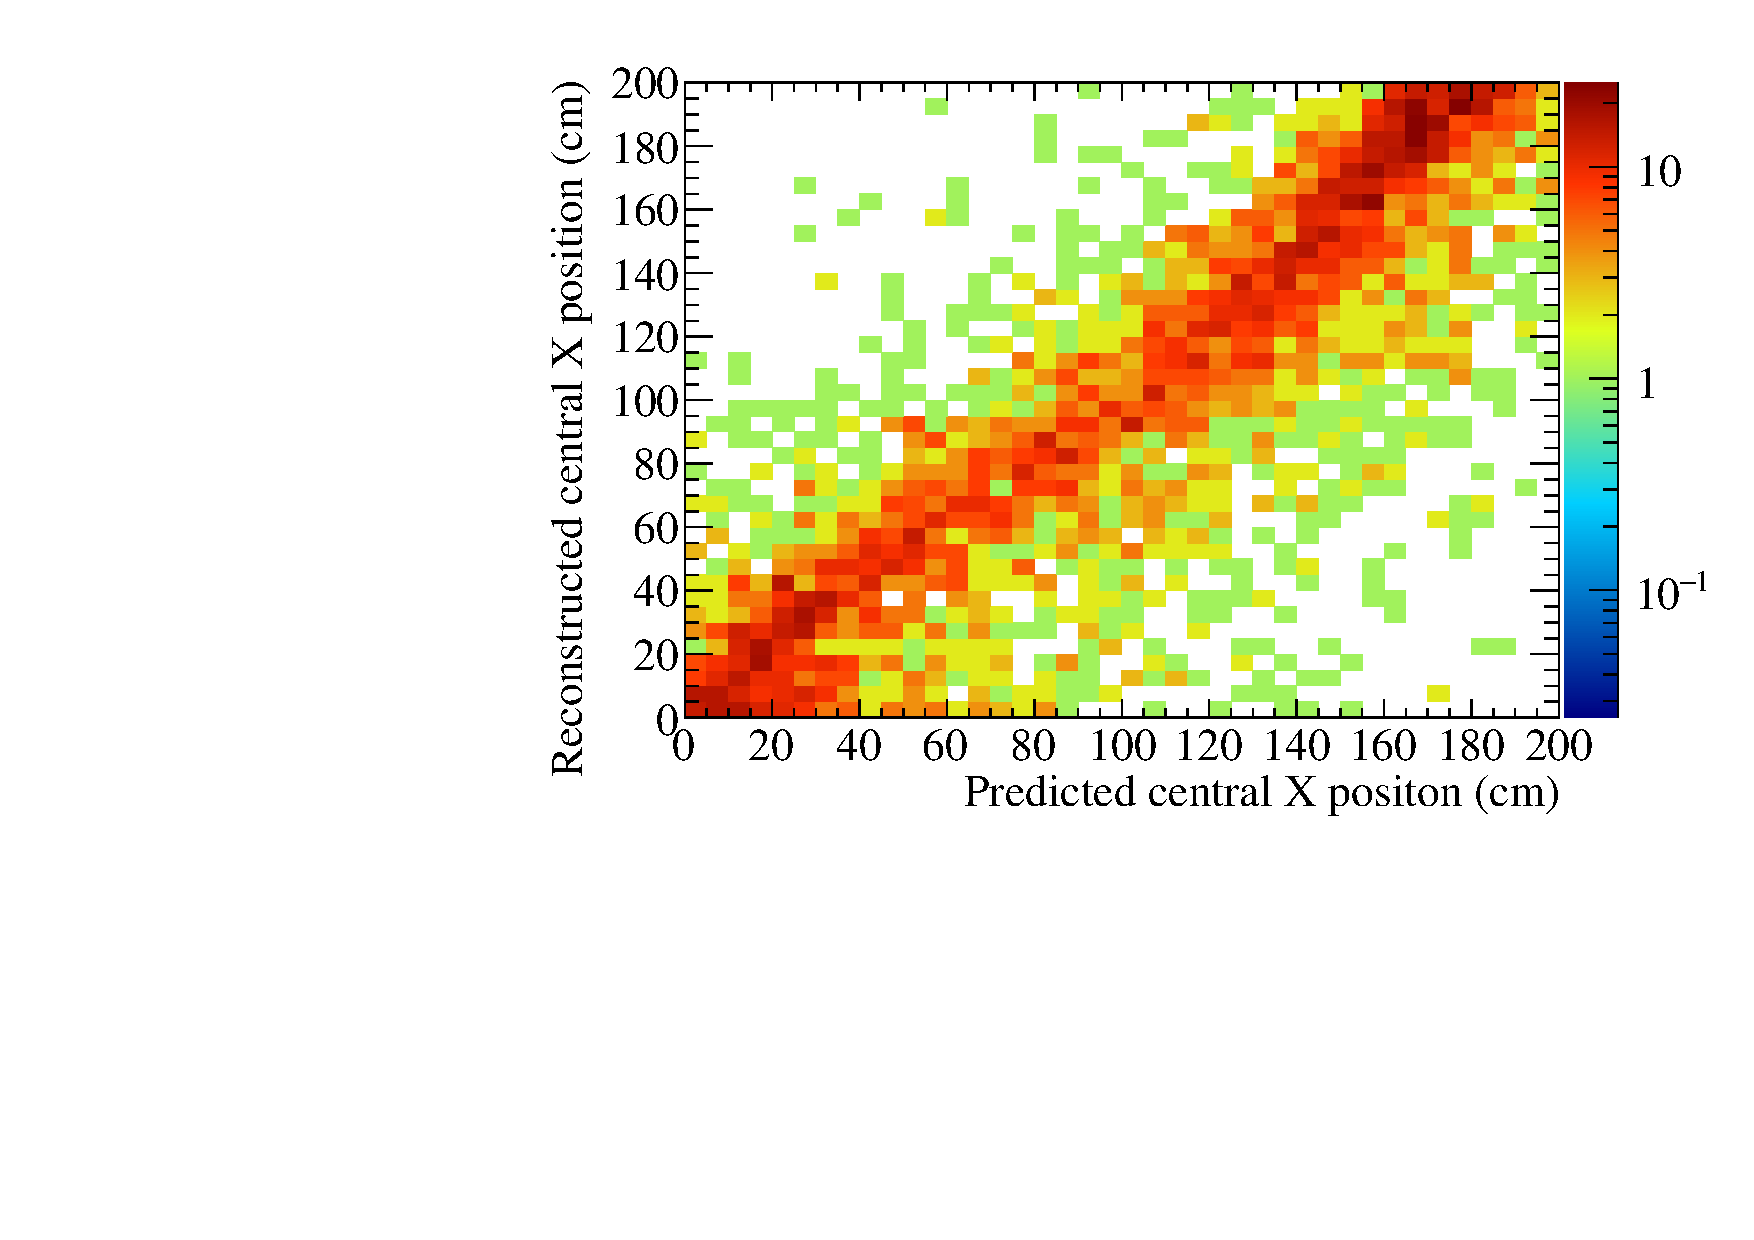
\includegraphics[width=0.6\textwidth]{DiffFlashPredReco}
  \caption[The predicted $x$ positions of flashes using the relationship between photoelectron and drift distance]
          {A comparison of the $x$ position predicted using the relationship in Fig~\ref{fig:NumPE_Distance}, and the $x$ position predicted using the difference in flash and hit times.}
  \label{fig:PD_PEDiffX}
\end{figure}

Using these metrics, it is possible to attempt to assign reconstructed flashes to reconstructed tracks. Only flashes which are within one drift window of a given track are considered, as flashes outside of this time window cannot have been caused by the reconstructed track. Once a flash has been assigned to a track, it is possible to determine how well the matching has performed, by comparing the Monte Carlo truth interaction time with the photon detector interaction time. When doing this, it is more useful to use a CRY sample which spans multiple drift windows, as then incoming particles will create scintillation flashes at random times, as opposed to all at $T$ = 0 as in the positive muon sample initially considered. The sample generated using CRY contains many particles, over a wide range of times, and is not limited to only producing positive muons. This means that it better represents the cosmic flux which will be observed by the 35 ton detector. The comparison between the Monte Carlo truth interaction time, and the photon detector interaction time, is shown in Figure~\ref{fig:PD_MCPDDiff}. \\

\begin{figure}
  \centering
  \begin{subfigure}{0.6\textwidth}
    \centering
    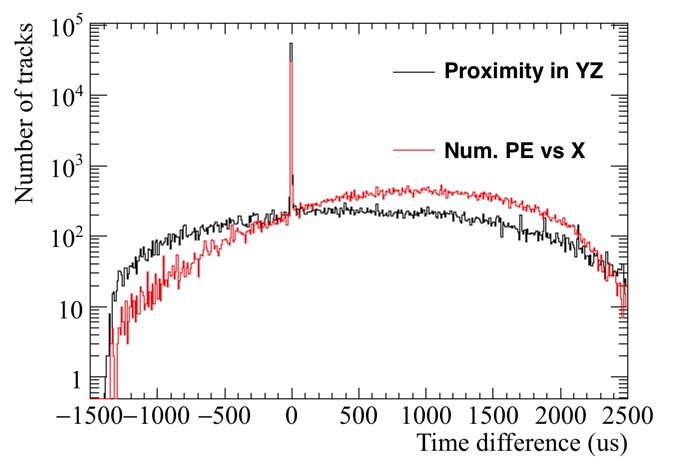
\includegraphics[width=\textwidth]{Pred_Reco_T_Full}
    \caption{The difference in interaction times.}
    \label{fig:PD_MCPDDiff_All}
  \end{subfigure}
  \begin{subfigure}{0.6\textwidth}
    \centering
    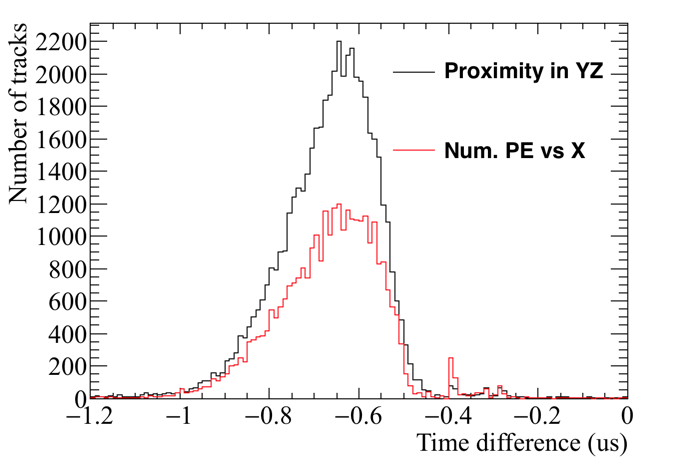
\includegraphics[width=\textwidth]{Pred_Reco_T_Zoom}
    \caption{Zoomed in at low time differences.}
    \label{fig:PD_MCPDDiff_Zoom}
  \end{subfigure}
  \caption[The number of events as a function of the difference between Monte Carlo and photon detector times]
          {The number of events as a function of the difference between Monte Carlo and photon detector times. Top: the difference in interaction times over a large range of times. Bottom: the peak at a time difference of 0 is expanded, showing a systematic offset of 0.6 $\mu$s due to an electronics offset in the simulation.}
          \label{fig:PD_MCPDDiff}
\end{figure}

Figure~\ref{fig:PD_MCPDDiff_All} shows a clear peak at a time difference of 0~ms between the Monte Carlo truth and photon detector times, showing that the interaction time which is calculated by the photon detectors is often very accurate. However, there is also a significant number of tracks for which the photon interaction time does not match the Monte Carlo truth interaction time. This is due to, for example, the broad width of the distribution shown in Figure~\ref{fig:NumPE_Distance}, meaning that the number of photoelectrons cannot necessarily accurately predict the distance between the APAs and the flash source. Improving the accuracy of the photon detector interaction time is required, as applying an incorrect interaction time correction will result in the $x$ position of hits being incorrect. The peak seen at a time difference of 0~ms has been expanded in Figure~\ref{fig:PD_MCPDDiff_Zoom}, where it can be seen that there is a systematic offset of 0.6 $\mu$s, this is due to an electronics offset applied in the simulation to the photon detector system. \\

From Figure~\ref{fig:PD_MCPDDiff} it can be seen that the metric using the proximity of the flash centre to the track trajectory, yields the best track/flash matches. This is likely caused by the large spread in the number of photoelectrons collected at fixed drift distances, as shown by Figure~\ref{fig:NumPE_Distance}, which causes a large degeneracy between the number of measured photoelectrons, and the distance between the APAs and the flash source. The two metrics can be combined to give a prediction for the interaction time, though given the increased sensitivity from the proximity metric, this should be given greater weighting. In physics data, the metric using the number of collected photoelectrons is particularly sensitive to the absolute light level in the detector. This is because a high residual light level in the detector would reduce the proportional change in the number of photoelectrons collected for increasing drift distances. This metric also relies on the existence of a sample of tracks with known $x$ positions, upon which to calibrate the change in the number of photoelectrons collected for increasing drift distances. It may be difficult to obtain this dataset in a real detector, though the cosmic ray counters around the 35 ton may be able to provide such a sample. \\

%********************************** % Second Section  *************************************
\section{Calibrating calorimetric constants} \label{sec:MCCalib} %Section - X.2
Having the correct calorimetric responses is vital when trying to calculate $\frac{dE}{dx}$, as the measured change in charge has to be correctly converted to the change in energy. The parameter which has to be tuned in order to ensure that this is done correctly, is the number of electrons that each ADC corresponds to. This was presented in Equations~\ref{eq:Birks} and~\ref{eq:ModBox}, as $C_{ADC \rightarrow e^{-}}$. Each plane will have a different response function, and so each plane has to be treated separately. These parameters have to be tuned in such a way as to make a known particle energy deposition have the correct $\frac{dE}{dx}$, the easiest deposition to tune against is the minimum ionising particle (MIP) peak, which in LAr should have a value of 1.8 MeV$\cdot$cm$^{-1}$. To do this, the sample of 10,000 positive muons made to calibrate the photon detector track/flash assignment will be used, as many of these particles will be MIPs. \\

To select the MIPs in the sample, only tracks caused by through-going muons are used. The $\frac{dE}{dx}$ value for all hits, in all tracks, is then calculated, and the different planes are considered separately. A Gaussian distribution is fitted around the peaks for each of the planes, to discern the Most Probable Value (MPV) of $\frac{dE}{dx}$ for that plane. If the MPVs are not equal to 1.8 MeV$\cdot$cm$^{-1}$, the ADC to electron parameters are scaled by the factor between the measured MPV and the MIP peak. As the relationship between $\frac{dE}{dx}$ and $C_{ADC \rightarrow e^{-}}$ is not linear, an element of trial and error is required to find the correct ADC to electron parameters. An example of the calibration being applied is shown in Figure~\ref{fig:CaloTune}. Calibration of the response functions is required whenever the electronics gains, or signal shaping functions, are changed.

\begin{figure}
  \centering
  \begin{subfigure}{0.6\textwidth}
    \centering
    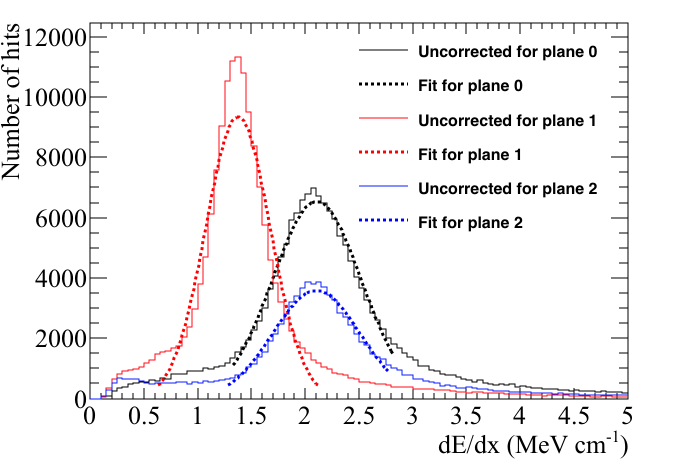
\includegraphics[width=\textwidth]{UnCorrectedCanvas}
    \caption{Before calibration is performed.}
    \label{fig:CaloTune_Before}
  \end{subfigure}
  \begin{subfigure}{0.6\textwidth}
    \centering
    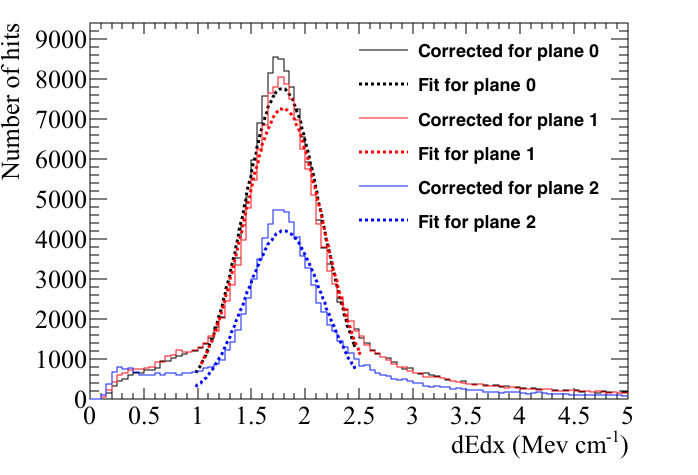
\includegraphics[width=\textwidth]{CorrectedCanvas}
    \caption{After calibration is performed.}
    \label{fig:CaloTune_After}
  \end{subfigure}
  \caption[The calibration of the calorimetric constants in the 35 ton]
          {The number of hits as a function the hit $\frac{dE}{dx}$, before and after calibration of the response functions for the conversion of ADC to number of electrons, for each plane. Top: the distribution of hit $\frac{dE}{dx}$ and the MPV of $\frac{dE}{dx}$ before calibration. Bottom: the distribution of hit $\frac{dE}{dx}$ and the MPV of $\frac{dE}{dx}$ after calibration. The collection plane, labelled as plane 2, is shown in blue, whilst the to induction planes, labelled plane 0 and plane 1, are shown in black and red respectively.}
          \label{fig:CaloTune}
\end{figure}
        
%********************************** % Third Section  *************************************
\section{Discerning reconstruction efficiencies} \label{sec:SimRecoEffic} %Section - X.3
Knowledge of the strengths and weaknesses of different tracking algorithms is vital when using them for physics analyses. To this end, it is useful to develop a metric by which they can be compared. In order to do this, a series of conditions have to be applied to the reconstructed tracks from a large set of simulated particles, which are reconstructed using different tracking algorithms. It is interesting to observe the effect that event complexity has on the reconstruction algorithms, and so efficiencies will be calculated for the positive muon sample, and the CRY sample, which were used in Section~\ref{sec:SimInteractionTimes}. The sample referred to as the positive muon sample contains single positive muons generated at $T$ = 0, with a constant $y$ position above the scintillation panels, and flat distributions in $x$ and $z$. The sample referred to as the CRY sample, contains multiple particles of multiple particle types generated at times spanning multiple drift windows, at zero altitude above sea level. \\

The criteria upon which to determine whether a particle is well reconstructed has to be carefully chosen, as every definition will have limitations. For example, consider a particle that travels 100~cm in the active volume of the detector, but is reconstructed as 2 separate tracks (tracks 1 and 2), with lengths 77~cm and 23~cm respectively. Firstly, should these tracks be merged, or left separate? If the reconstruction algorithms have found them to be separate tracks, then it is likely that it would be difficult to ascertain that they are from the same particle in real data, and so in considerations here they are not merged. Secondly, one has to determine what the definition of a well reconstructed track should be. One definition of a well reconstructed track, would be that the reconstructed track length is between 75$\%$ and 125$\%$ of the track length in the detector from Monte Carlo truth, in which case track 1 would be considered well reconstructed. Another definition to consider however, would be whether the track length in the detector from Monte Carlo truth is between 75$\%$ and 125$\%$ of the reconstructed track length, in which case neither track would be considered well reconstructed. These definitions have used exactly the same tracks, and seemingly identical definitions of what constitutes a well reconstructed track, but they have got very different results. As such, it is wrong to say which definition gives the correct result, but instead the result of each should be considered equally. It should also be noted, that these are just two of a wide range of definitions one could use to quantify whether a track is well reconstructed. In the discussions presented here, the former definition of a well reconstructed track is used, such that a track is considered well reconstructed if:
\begin{itemize}
\item The reconstructed track length is more than or equal to 75$\%$ of the Monte Carlo track length.
\item The reconstructed track length is less than or equal to 125$\%$ of the Monte Carlo track length.
\item Only one reconstructed track can be matched per Monte Carlo particle.
\end{itemize}
When calculating the reconstruction efficiencies, the number of well reconstructed tracks, is divided by the total number of particles in the active volume, from Monte Carlo truth. When calculating these efficiencies, it is important to consider much more than just the Monte Carlo truth track length. To this end, efficiencies with regards to several parameters of the tracks are calculated:
\begin{itemize}
\item Track length,
\item Energy deposited in the active volume of the detector,
\item The angle $\theta$ of the track, defined as the angle that a vector makes from the $x$ axis in the $xy$ plane,
\item The angle $\phi$ of the track, defined as the angle between the $z$ axis and the vector.
\end{itemize}
In all efficiency plots, the Monte Carlo truth quantity, not the reconstructed quantity, is shown, so as to reflect how the change in these quantities affects the reconstruction efficiency. It is also useful to observe the effect that failed disambiguation, and incorrect interaction time determination, has on the reconstruction efficiency. To show this, two reconstruction paths are ran on the particles. One reconstruction path uses no Monte Carlo information, and so the disambiguation is performed as outlined in Section~\ref{sec:LArSoft}, and the interaction time is determined using the simulated photon detectors, as described in Section~\ref{sec:SimInteractionTimes}. The second reconstruction path uses ``cheated disambiguation,'' whereby Monte Carlo truth information is used to select the wire segments which hits occurred on, and Monte Carlo truth information is also used when calculating the interaction time of the track. \\

The calculation of reconstruction efficiencies also serves as an effective method upon which reconstruction algorithms can be further developed, as it identifies aspects which do not work as expected. For example, when the reconstruction efficiencies for the CRY sample were initially calculated, they were significantly lower than for the positive muon sample (at 10\%), but only when disambiguation was not cheated. It transpired that this was because the disambiguation was only selecting the largest collection of hits on each plane, for each TPC. This is not a problem when only 1 particle is simulated, as one would expect that there only be one particle on a given plane, in each TPC. However, when considering a CRY sample which lasts of the order of 10~ms, there will almost certainly be multiple particles on each plane, in each TPC. Removing the hits from all but one of these multiple particles, will cause them to have no reconstructed track, and thus cause the efficiency to drop significantly. Upon making the disambiguation algorithm no longer have this restriction, the reconstruction efficiencies of the positive muon and CRY samples were observed to become much more similar, as presented here. \\

The reconstruction efficiencies given the current state of the most commonly used reconstruction algorithms, Pandora~\citep{Pandora} and PMTrack~\citep{PMTrack}, are shown in Figures~\ref{fig:SimEffic_Length},~\ref{fig:SimEffic_EnDepos},~\ref{fig:SimEffic_Theta},~\ref{fig:SimEffic_Phi} and~\ref{fig:SimEffic_ThetaPhi}. Efficiencies are shown for both the positive muon and CRY samples, where it can be seen that the efficiency tends to be lower for the CRY sample. It is thought that this is due to the more complex event structure in the CRY sample, as multiple primary particles will be present in the detector at any given time. The relatively slow drift velocity of LAr may mean that these tracks cross in wire-tick space. Tracks crossing in wire-tick space could cause reconstruction errors, as the overlaps may be mistaken for interactions, which would cause the tracks to be split, resulting in the interaction time calculated from the photon detectors to be incorrect. This error, in the calculation of interaction time using the photon detectors, was seen in Figure~\ref{fig:PD_MCPDDiff}. The reconstruction efficiencies for the CRY sample are more realistic, as events will rarely be isolated in the 35 ton detector, due to the large flux of cosmic particles on the Earth's surface. \\

\begin{figure}
  \centering
  \begin{subfigure}{0.48\textwidth}
    \centering
    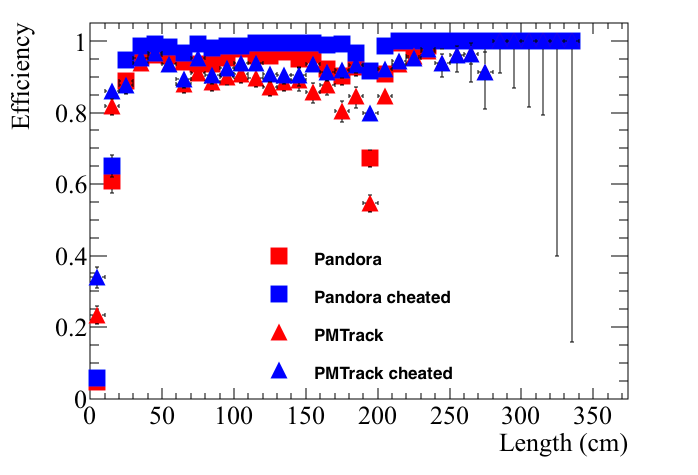
\includegraphics[width=\textwidth]{Effic_AntiMuon_500V_All_Length}
    \caption{Reconstruction efficiencies for the positive muon sample.}
    \label{fig:SimEffic_Length_AMu}
  \end{subfigure}%
  \hspace{0.03\textwidth}%
  \begin{subfigure}{0.48\textwidth}
    \centering
    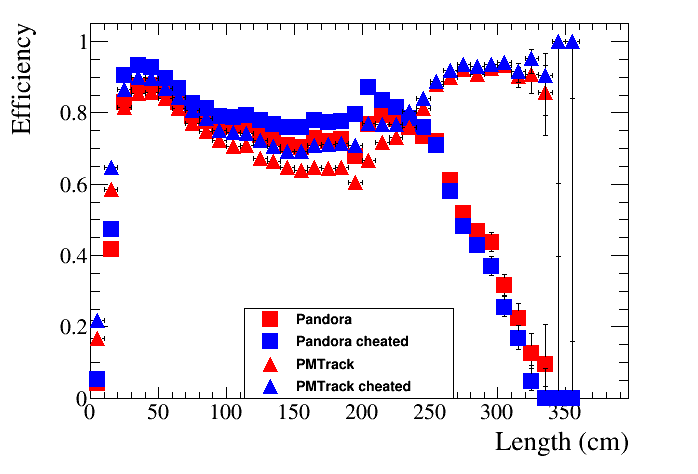
\includegraphics[width=\textwidth]{Effic_Cosmics_500V_All_Length}
    \caption{Reconstruction efficiencies for the CRY sample.}
    \label{fig:SimEffic_Length_CRY}
  \end{subfigure}
  \caption[The reconstruction efficiencies for simulated events as a function of the track length in the detector from Monte Carlo truth.]
          {The reconstruction efficiencies for simulated events as a function of the track length in the detector from Monte Carlo truth. The efficiencies are shown for ``non-cheated'' reconstruction (red), and ``cheated'' reconstruction (blue), for both Pandora~\citep{Pandora} (squares) and PMTrack~\citep{PMTrack} (triangles).}
          \label{fig:SimEffic_Length}
\end{figure}

\begin{figure}
  \centering
  \begin{subfigure}{0.48\textwidth}
    \centering
    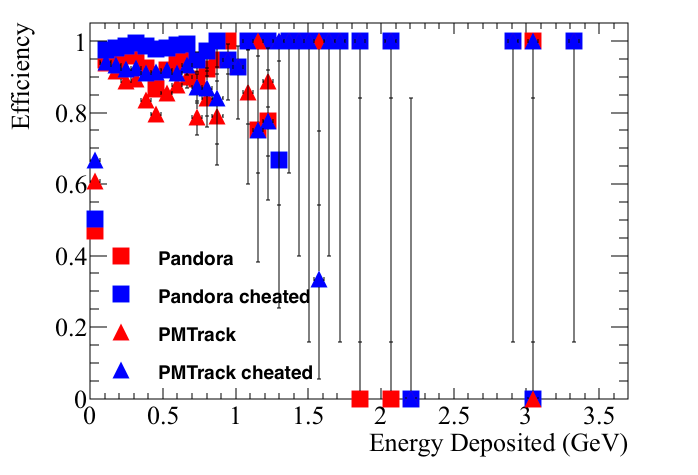
\includegraphics[width=\textwidth]{Effic_AntiMuon_500V_All_EnDepos}
    \caption{Reconstruction efficiencies for the positive muon sample.}
    \label{fig:SimEffic_EnDepos_AMu}
  \end{subfigure}%
  \hspace{0.03\textwidth}%
  \begin{subfigure}{0.48\textwidth}
    \centering
    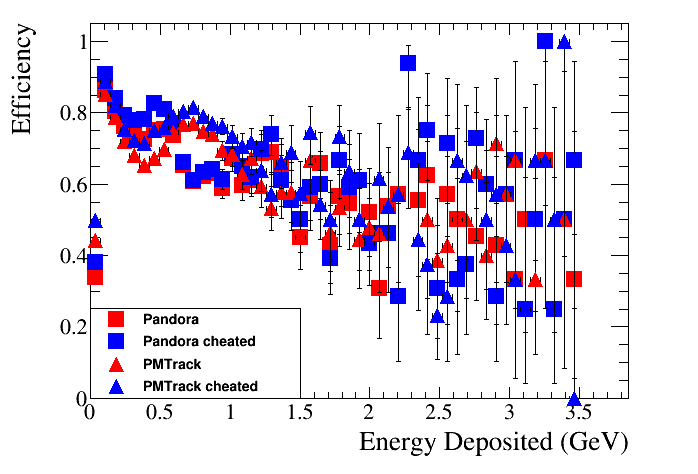
\includegraphics[width=\textwidth]{Effic_Cosmics_500V_All_EnDepos}
    \caption{Reconstruction efficiencies for the CRY sample.}
    \label{fig:SimEffic_EnDepos_CRY}
  \end{subfigure}
  \caption[The reconstruction efficiencies for simulated events as a function of the deposited energy from Monte Carlo truth.]
          {The reconstruction efficiencies for simulated events as a function of the deposited energy from Monte Carlo truth. The efficiencies are shown for ``non-cheated'' reconstruction (red), and ``cheated'' reconstruction (blue), for both Pandora~\citep{Pandora} (squares) and PMTrack~\citep{PMTrack} (triangles).}
          \label{fig:SimEffic_EnDepos}
\end{figure}

\begin{figure}
  \centering
  \begin{subfigure}{0.48\textwidth}
    \centering
    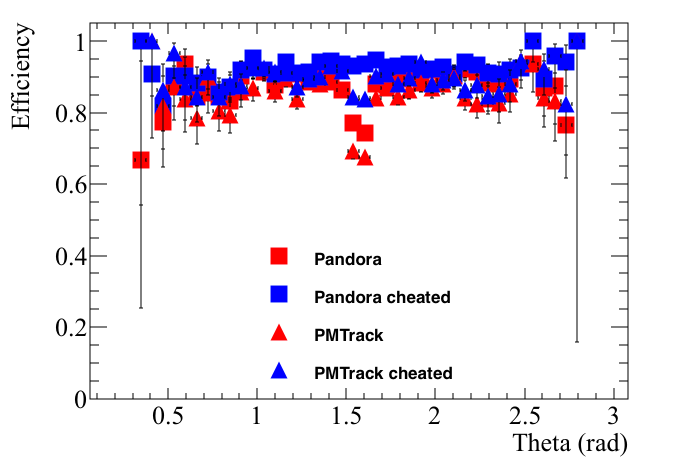
\includegraphics[width=\textwidth]{Effic_AntiMuon_500V_All_Theta}
    \caption{Reconstruction efficiencies for the positive muon sample.}
    \label{fig:SimEffic_Theta_AMu}
  \end{subfigure}%
  \hspace{0.03\textwidth}%
  \begin{subfigure}{0.48\textwidth}
    \centering
    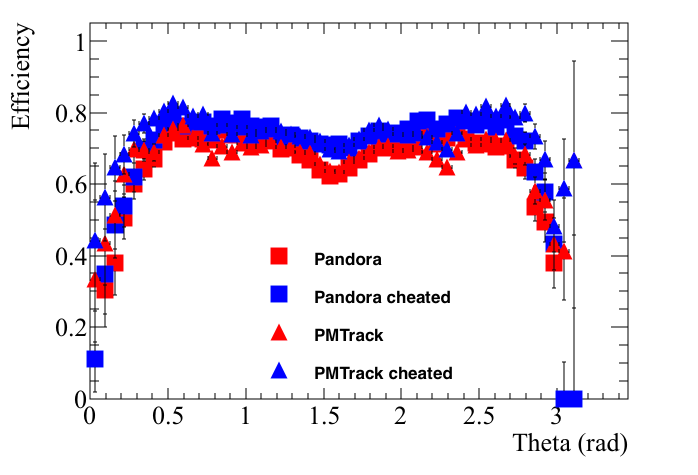
\includegraphics[width=\textwidth]{Effic_Cosmics_500V_All_Theta}
    \caption{Reconstruction efficiencies for the CRY sample.}
    \label{fig:SimEffic_Theta_CRY}
  \end{subfigure}
  \caption[The reconstruction efficiencies for simulated events as a function of the $\theta$ track angle from Monte Carlo truth track.]
          {The reconstruction efficiencies for simulated events as a function of the $\theta$ track angle from Monte Carlo truth track. The efficiencies are shown for ``non-cheated'' reconstruction (red), and ``cheated'' reconstruction (blue), for both Pandora~\citep{Pandora} (squares) and PMTrack~\citep{PMTrack} (triangles).}
          \label{fig:SimEffic_Theta}
\end{figure}

\begin{figure}
  \centering
  \begin{subfigure}{0.48\textwidth}
    \centering
    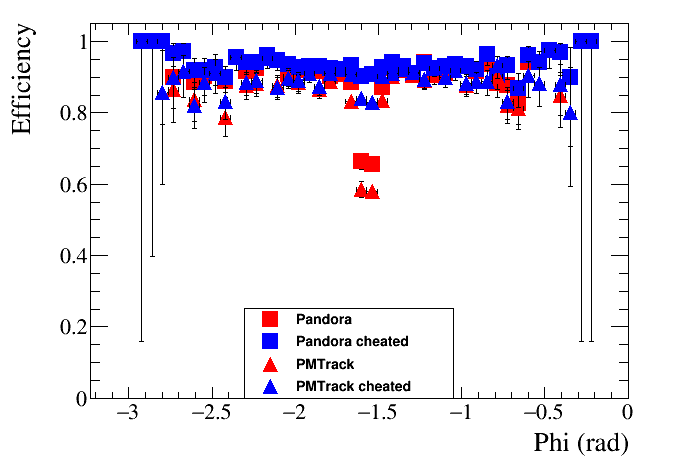
\includegraphics[width=\textwidth]{Effic_AntiMuon_500V_All_Phi}
    \caption{Reconstruction efficiencies for the positive muon sample.}
    \label{fig:SimEffic_Phi_AMu}
  \end{subfigure}%
  \hspace{0.03\textwidth}%
  \begin{subfigure}{0.48\textwidth}
    \centering
    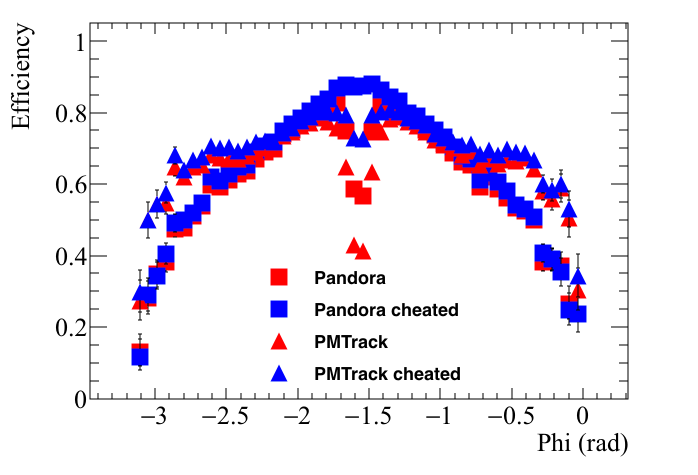
\includegraphics[width=\textwidth]{Effic_Cosmics_500V_All_Phi}
    \caption{Reconstruction efficiencies for the CRY sample.}
    \label{fig:SimEffic_Phi_CRY}
  \end{subfigure}
  \caption[The reconstruction efficiencies for simulated events as a function of the $\phi$ track angle from Monte Carlo truth track.]
          {The reconstruction efficiencies for simulated events as a function of the $\phi$ track angle from Monte Carlo truth track. The efficiencies are shown for ``non-cheated'' reconstruction (red), and ``cheated'' reconstruction (blue), for both Pandora~\citep{Pandora} (squares) and PMTrack~\citep{PMTrack} (triangles).}
          \label{fig:SimEffic_Phi}
\end{figure}

\begin{figure}
  \centering
  \begin{subfigure}{0.8\textwidth}
    \centering
    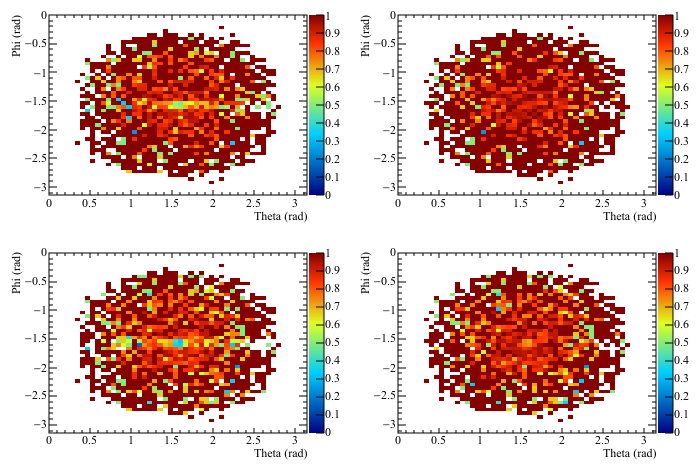
\includegraphics[width=\textwidth]{Effic_AntiMuon_500V_All_PhiTheta}
    \caption{Reconstruction efficiencies for the positive muon sample.}
    \label{fig:SimEffic_ThetaPhi_AMu}
  \end{subfigure}
  \begin{subfigure}{0.8\textwidth}
    \centering
    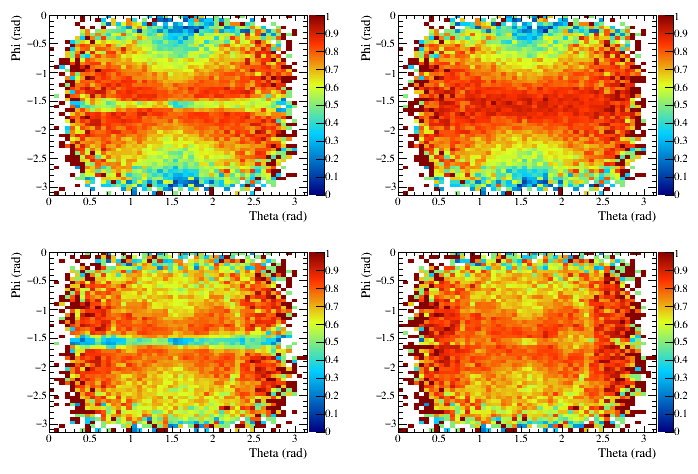
\includegraphics[width=\textwidth]{Effic_Cosmics_500V_All_PhiTheta}
    \caption{Reconstruction efficiencies for the CRY sample.}
    \label{fig:SimEffic_ThetaPhi_CRY}
  \end{subfigure}
  \caption[The reconstruction efficiencies for simulated events as a function of the $\theta$ and $\phi$ track angles from Monte Carlo truth track.]
          {The reconstruction efficiencies for simulated events as a function of the $\theta$ and $\phi$ track angles from Monte Carlo truth track. The track angle $\theta$ is shown on the $x$ axis, and the track angle $\phi$ is shown on the $y$ axis. The colour $z$ axis shows the reconstruction efficiency. In both figures, ``normal'' (left) and ``cheated'' (right) disambiguation is shown, for both Pandora~\citep{Pandora} (top) and PMTrack~\citep{PMTrack} (bottom).}
          \label{fig:SimEffic_ThetaPhi}
\end{figure}

A striking feature of Figure~\ref{fig:SimEffic_Length} is the rapid decrease in reconstruction efficiency seen in the CRY sample, for particles with track lengths in the detector of more than 250~cm from Monte Carlo truth, when using Pandora. The cause of this, is that tracks are reconstructed separately in the long, and short drift volumes, before being merged when they are found to be co-linear in the $yz$ plane. This is not a problem in the positive muon sample, as the $x$ position of the hits calculated using Equation~\ref{eq:HitTime} will be correct.
\begin{equation}
   \label{eq:HitTime}
   x_{Hit} = T_{Hit} \times \text{v}_{Drift}
\end{equation}
In Equation~\ref{eq:HitTime}, $x_{Hit}$ is the calculated $x$ position of the hit, $T_{Hit}$ is the measured time of the hit, and v$_{Drift}$ is the electron drift velocity. An electron, in an electric field of 500~V$\cdot$cm$^{-1}$, in LAr, drifts at a speed of 0.160563~cm$\cdot\mu$s$^{-1}$. However, when the same is done for hits in the CRY sample, using particles with large interaction times, the $x$ positions will have offsets proportional to the interaction time of the particle, unless the hit time is corrected by Equation~\ref{eq:HitTime_Int}.
\begin{equation}
   \label{eq:HitTime_Int}
   T_{Hit} = T_{Measured} - T_{Interaction}
\end{equation}
In Equation~\ref{eq:HitTime_Int}, $T_{Hit}$ is the corrected hit time, $T_{Measured}$ is the measured time of the hit, and $T_{Interaction}$ is the calculated interaction of the particle which caused the hit. \\

The scale of these offsets in $x$ positions can be seen by considering a particle which is generated at a time of $T$ = 12.5~ms, as then the offset in the reconstructed $x$ position calculated by Equation~\ref{eq:HitTime}, would be more than 20 m! Obviously the hits could not have occurred at these positions, as the drift distances are roughly 30~cm in the ``short'' drift volume, and 225~cm in the ``long'' drift volume. However, as track segments are reconstructed separately in the ``short'' and ``long'' drift volumes, before later being merged, it is possible for there to be a discontinuity in $x$ of more than 40 m, if these $x$ offsets are not corrected for. As the interaction time of the track is calculated using the output of the tracking algorithms, it is not possible to prevent this by using the interaction time at present. It is however, possible to subtract this discontinuity in $x$ from the total reconstructed track length when the stitched track is stored in the event. This will give the correct track length, though the user will still have to correct the positions of individual hits, using the calculated interaction times. This is what is done by PMTrack, hence it not exhibiting this rapid decrease in reconstruction efficiency for long tracks. The interaction time can be found from, among other things, the Monte Carlo truth generation time, or the photon detectors, as discussed in Section~\ref{sec:SimInteractionTimes}.\\

It is clear from Figure~\ref{fig:SimEffic_Length} that particles with track lengths in the detector of less than 30~cm are poorly reconstructed. The extremely low efficiency for particles with track lengths of less than 10~cm, can be partially attributed to particles with track lengths of less than 1~cm in the active volume of the detector. These particles, which represent 30\% of the particles with active volume track lengths of less than 10~cm, are too short to be reconstructed using the current reconstruction process. These particles will need to be reconstructed when looking for supernovae bursts, though special algorithms will be written to do this, as the traditional hit finding and clustering algorithms may discard them due to the isolated nature of the hits. Another issue, is that the low energies of these particles may mean that the signals that they produce are below threshold, and so will not even be reconstructed, or, if hits are reconstructed, they may be too close to a more energetic track and get absorbed into them. The reconstruction of tracks is affected by the number of wires which they cross, though this should not matter for particles with track lengths of more than 5~cm in the active volume, as they will have crossed roughly 10 wires in each plane, which should produce enough unique hits for a cluster to be reliably reconstructed. This can be seen to be the case for PMTrack when considering the positive muon sample, as the efficiency for particle track lengths between 10 and 20~cm, is roughly the same as that for track lengths between 20 and 30~cm. However, when considering the CRY sample, there is still a significant decrease in efficiency. This is attributed to secondary particles which are produced in hadronic interactions with the concrete surrounding the detector. Many of these particles will travel only very short distances in the active volume, though those that travel slightly larger distances are likely to cause energy depositions that will be confined to the detector edges. The tracking algorithms may struggle to accurately reconstruct these tracks, as significant portions of the track will be close to the detector edge, where the field is poorly modelled, and hits may be more difficult to disambiguate. \\

The trend of increasing efficiency for longer track lengths, which was seen in Figure~\ref{fig:SimEffic_Length}, can also be seen in Figure~\ref{fig:SimEffic_EnDepos}, where the reconstruction efficiency increases as the amount of deposited energy increases. This is because particles which deposit more energy, will tend to have travelled further in the detector. The amount of energy that particles deposit is limited by the size of the detector, as particles with an energy of more than 1 GeV are energetic enough to be MIPs. This results in few particles depositing more than 1 GeV in the detector, and is why the uncertainty in the reconstruction efficiency increases for energy depositions in the detector volume of more than 1 GeV. The larger range in the amount of energy deposited seen in Figure~\ref{fig:SimEffic_EnDepos_CRY}, is due to the larger number of muons in the CRY sample which create large electromagnetic showers upon entering the LAr. \\

It is also interesting to note the pronounced decreases in reconstruction efficiencies for particular angles, shown in Figures~\ref{fig:SimEffic_Theta} and~\ref{fig:SimEffic_Phi}. The decrease in efficiency at $\phi = \frac{\pi}{2}$, seen in Figure~\ref{fig:SimEffic_Phi}, can be attributed to the drop in efficiency for particles with track lengths between 190~cm and 200~cm, seen in Figure~\ref{fig:SimEffic_Length}. This is because the vertical height of the detector is approximately 195~cm, and near vertical tracks will hit few collection wires, meaning that determining the triple points needed by the disambiguation is very difficult. This is verified by the large increase in efficiency achieved by cheating the disambiguation, as seen in Figure~\ref{fig:SimEffic_Theta_AMu}, where the reduction in reconstruction efficiency is seen to become much less pronounced. Similarly, the decrease in efficiency at $\theta = \frac{\pi}{2}$ can be attributed to particles which are perpendicular to the collection plane wires, as this track orientation also results in few collection wires being hit. \\  

The information from Figures~\ref{fig:SimEffic_Theta} and~\ref{fig:SimEffic_Phi} is combined in Figure~\ref{fig:SimEffic_ThetaPhi}, where the sharp drop in efficiency at $\phi = \frac{\pi}{2}$ for the ``non-cheated'' CRY sample is particularly visible. The effect of cheated disambiguation is clear in Figure~\ref{fig:SimEffic_ThetaPhi_CRY}, where the dip in efficiency as a function of $\theta$ at fixed $\phi=\frac{\pi}{2}$ is completely removed. The same is not true however, for the dip in efficiency as a function $\phi$ at fixed $\theta = \frac{\pi}{2}$, though the reduction in efficiency was not as severe as that seen for fixed values of $\phi = \frac{\pi}{2}$. The effect of ``cheated disambiguation'' can still be seen though, as the reconstruction efficiency in Figure~\ref{fig:SimEffic_ThetaPhi_CRY} can be seen to improve for values of $\phi$. There are still however, noticeable decreases in the reconstruction efficiency for values of $\phi$ close to 0 or $\pi$, when using Pandora. The improvement in the performance of the reconstruction algorithms that comes from ``cheating'' the reconstruction, is part of the motivation for the wire pitches in the DUNE FD being 36$^{\circ}$, as opposed to the 45$\pm$0.7$^{\circ}$ used in the 35 ton. This is because, as discussed in Section~\ref{sec:LArSoft}, the shallower wire pitch makes disambiguation easier. Though disambiguation will be easier in the different geometry, further efforts to improve disambiguation are still required, as are continued efforts to reconstruct the shortest tracks. \\

%********************************** % Fourth Section  *************************************
\section{Performing particle identification}  \label{sec:PID} %Section - X.4
Being able to perform reliable Particle IDentification (PID) is a key requirement for the DUNE experiment, and so efforts have been made to establish a procedure by which this can be achieved. The predominant method of performing PID in LAr is to use the relationship between $\frac{dE}{dx}$, and the residual range of the track. The residual range of a track is defined as, the distance between a given point on the track and the stopping point of the track. This relationship depends on particle for small values of $\beta$, and is quantified by the Bethe-Bloch equation~\citep{Bethe, Bloch} which is shown in Figure~\ref{fig:BetheBloch}, and presented in Equation~\ref{eq:Bethe-Bloch}. \\

\begin{figure}
  \centering
  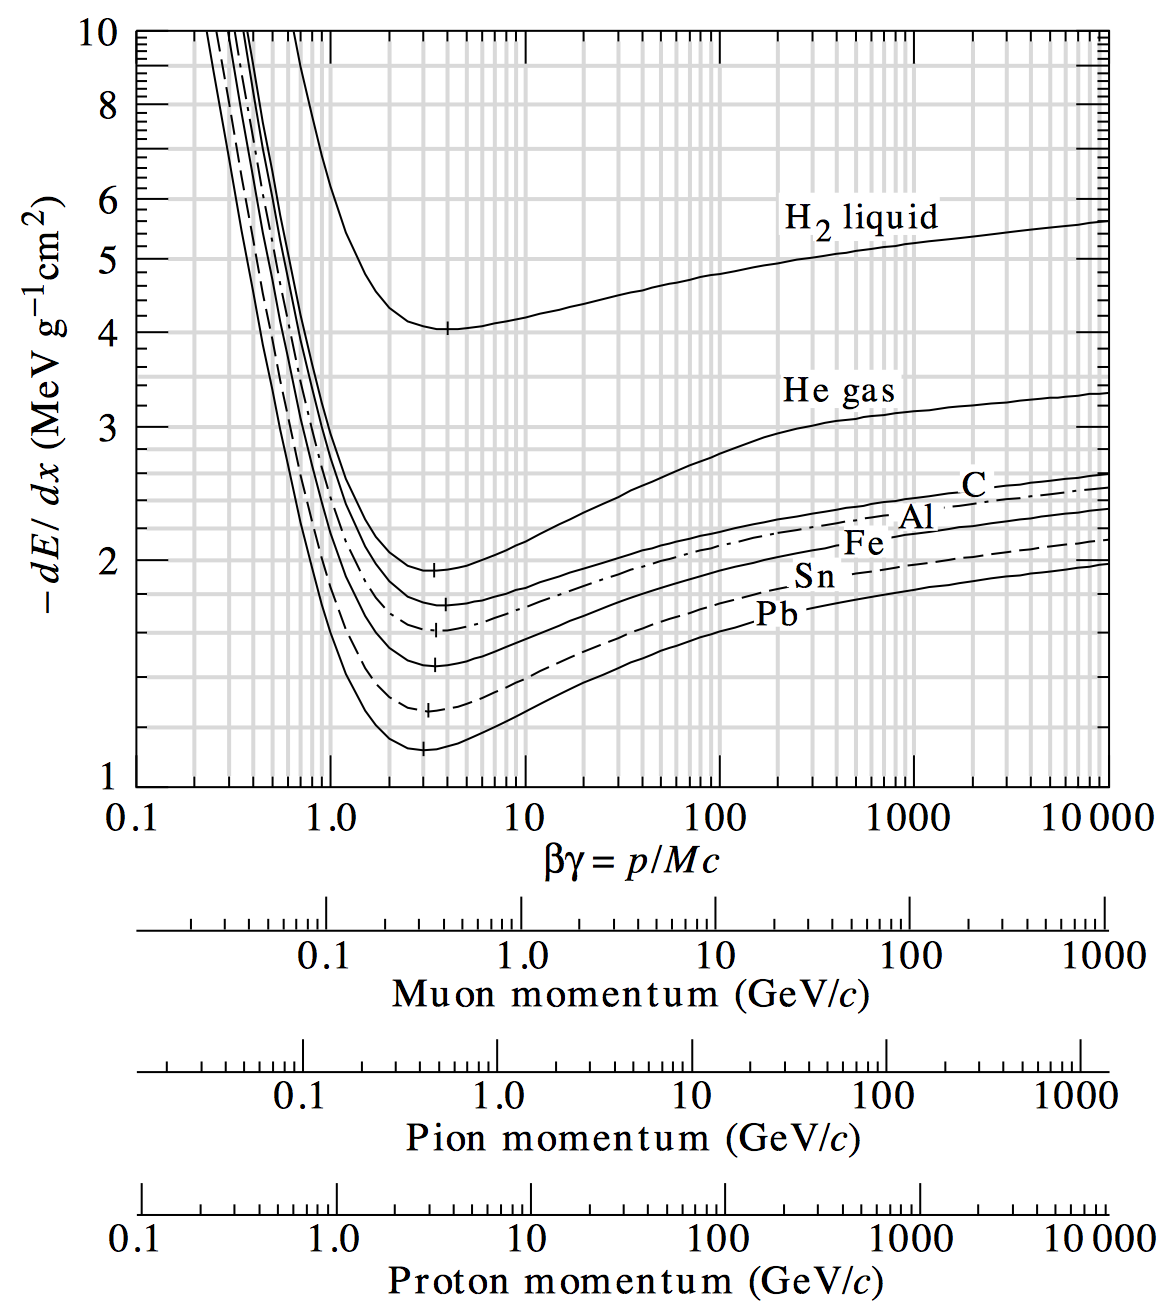
\includegraphics[width=0.5\textwidth]{Bethe-Bloch}
  \caption[The mean energy loss per unit track length of different particle masses in different materials]
          {The mean energy loss per unit track length of different particle masses in different materials~\citep{PDGReview}. The $\frac{Z}{A}$ of liquid argon is slightly less than that of carbon.}
  \label{fig:BetheBloch}
\end{figure}

\begin{equation}
  \label{eq:Bethe-Bloch}
  -\frac{dE}{dx} = K z^2 \frac{Z}{A} \frac{1}{\beta^2} \left[ \frac{1}{2} \ln{\frac{2 m_e c^2 \beta^2 \gamma^2 T_{max}}{I^2}} - \beta^2 - \frac{\delta(\beta\gamma)}{2}\right]
\end{equation}
where $K = 4 \pi N_A r_{e}^{2} m_e c^2$, $N_A$ is Avogadro's number, $r_e$ is the radius of the electron, $m_e$ is the electron mass, $z$ is the charge of the particle, $Z$ is the atomic number of the material, $A$ is the atomic mass of the material, $T_{max}$ is the maximum energy transferred to the ionisation electron, $I$ is the mean excitation energy, and $\delta(\beta\gamma)$ is the density effect correction to ionisation energy loss. \\

The sharp increase in energy loss per unit length can be seen to occur at different momenta for different particle masses in Figure~\ref{fig:BetheBloch}, meaning that the peak value of $\frac{dE}{dx}$ changes significantly for particles of different masses. For example, it can be seen that the momenta at which the increase in $\frac{dE}{dx}$ occurs is very different for muons and protons. However, it can be seen the momenta at which this increase in $\frac{dE}{dx}$ occurs is very similar when considering muons and pions. For this reason, it should be relatively simple to discern a proton track from a muon track, though it may be difficult to discern a muon track from a pion track. \\

The particle mass dependence can be seen by plotting the $\frac{dE}{dx}$ against the residual range of the particle on a log-log plot, as shown in Figure~\ref{fig:PIDA_loglog}. A power law dependence is found to describe the relationship~\citep{PIDA_Paper}, as shown in Equation~\ref{eq:PIDA}.
\begin{equation}
  \label{eq:PIDA}
  \frac{dE}{dx} = A R^b
\end{equation}
where $A$ and $b$ are constants for a particle and a given material. The dependence on $b$ is found to be weak, and so can be set to -0.42 for all particle masses. This means that the main discriminant used is the $A$ parameter, which has a strong dependence on particle mass. Table~\ref{tab:PIDAVals} shows the values of $A$ and $b$ which are calculated from Figure~\ref{fig:PIDA_loglog}. It is found that the error introduced by fixing the $b$ parameter is small compared to the error from ionisation fluctuations~\citep{PIDA_Paper}. \\

\begin{table}
\caption[Stopping power parameterisation for various particle types in liquid argon]
        {Stopping power parameterisation for various particle types in liquid argon. The table is taken from~\citep{PIDA_Paper}.}
\centering
\label{tab:PIDAVals}
\begin{tabular}{l c c}
\toprule
{Particle} & {A (MeV$\cdot$cm$^{b-1}$)} & {b} \\ 
\midrule
Pion     & 8  & -0.37 \\

Kaon     & 14 & -0.41 \\

Proton   & 17 & -0.42 \\

Deuteron & 25 & -0.43 \\
\bottomrule
\end{tabular}
\end{table}

Once the $b$ parameter is set to be constant for all particle types, it is possible to calculate a value of the $A$ parameter for each hit on the track using Equation~\ref{eq:PIDA_A}, where $R_i$ is the residual range of the track at that point.
\begin{equation}
  \label{eq:PIDA_A}
  A_i = \left(\frac{dE}{dx}\right)_i \times \left(R_{i}\right)^{0.42}
\end{equation}
The particle type discriminant, called PIDA, can then be calculated for a track by finding the average value of $A_i$ for the track. As the particle mass dependant increase in $\frac{dE}{dx}$ only occurs near the end of the track, the PIDA variable can only be calculated for particles which stop in the detector, as all other particles will have MIP-like $\frac{dE}{dx}$ distributions and so cannot be identified in this way. As shown by the plotted range of Figure~\ref{fig:PIDA_loglog}, the average value of $A$ is normally calculated for the last 30~cm of the track. \\

\begin{figure}
  \centering
  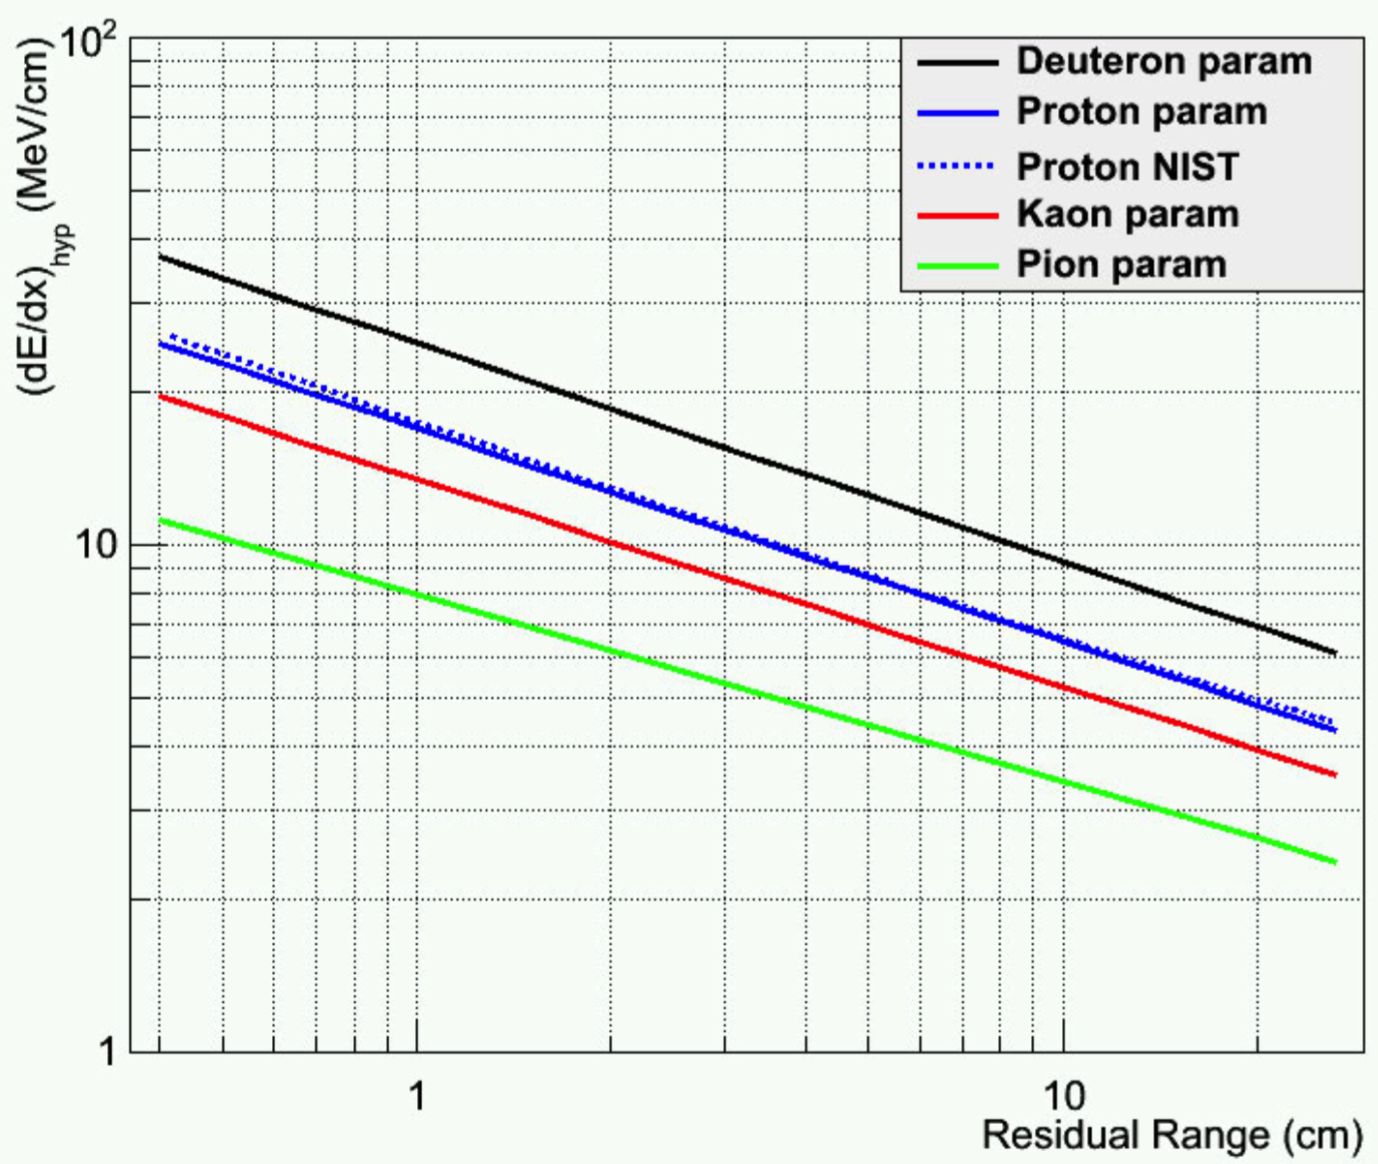
\includegraphics[width=0.5\textwidth]{StoppingPower}
  \caption[Stopping power for different particle masses as a function of residual range in liquid argon]
          {Stopping power for different particle masses as a function of residual range in liquid argon. The figure is taken from~\citep{PIDA_Paper}.}
  \label{fig:PIDA_loglog}
\end{figure}

The PIDA method was tested in~\citep{PIDA_Paper}, where the PIDA values were calculated for simulated particles which stopped in the detector, using Monte Carlo truth information over the last 30~cm of the particle tracks. This is shown in Figure~\ref{fig:PIDA_MC}, where a clear separation can be seen between the peaks for muons, pions, kaons, and protons. Though the muon and pion peaks are relatively close together, they can still be resolved in the plot due to little overlap. It is interesting to note how tight the PIDA distributions found in the paper are, which allows the different particles types to cleanly separated in the truth study. An incorrect tuning of the electron recombination effects will cause the distributions in Figure~\ref{fig:PIDA_MC} to become broader~\citep{PIDA_Paper}. The dependence of $\frac{dE}{dx}$ on the recombination effects ($Recomb_{A/B}$) were presented in Equations~\ref{eq:Birks} and~\ref{eq:ModBox}. Also, an incorrect calibration of the detector will introduce a systematic shift in the expected values of PIDA~\citep{PIDA_Paper}, this is why the work presented in Section~\ref{sec:MCCalib} is important. \\

\begin{figure}
  \centering
  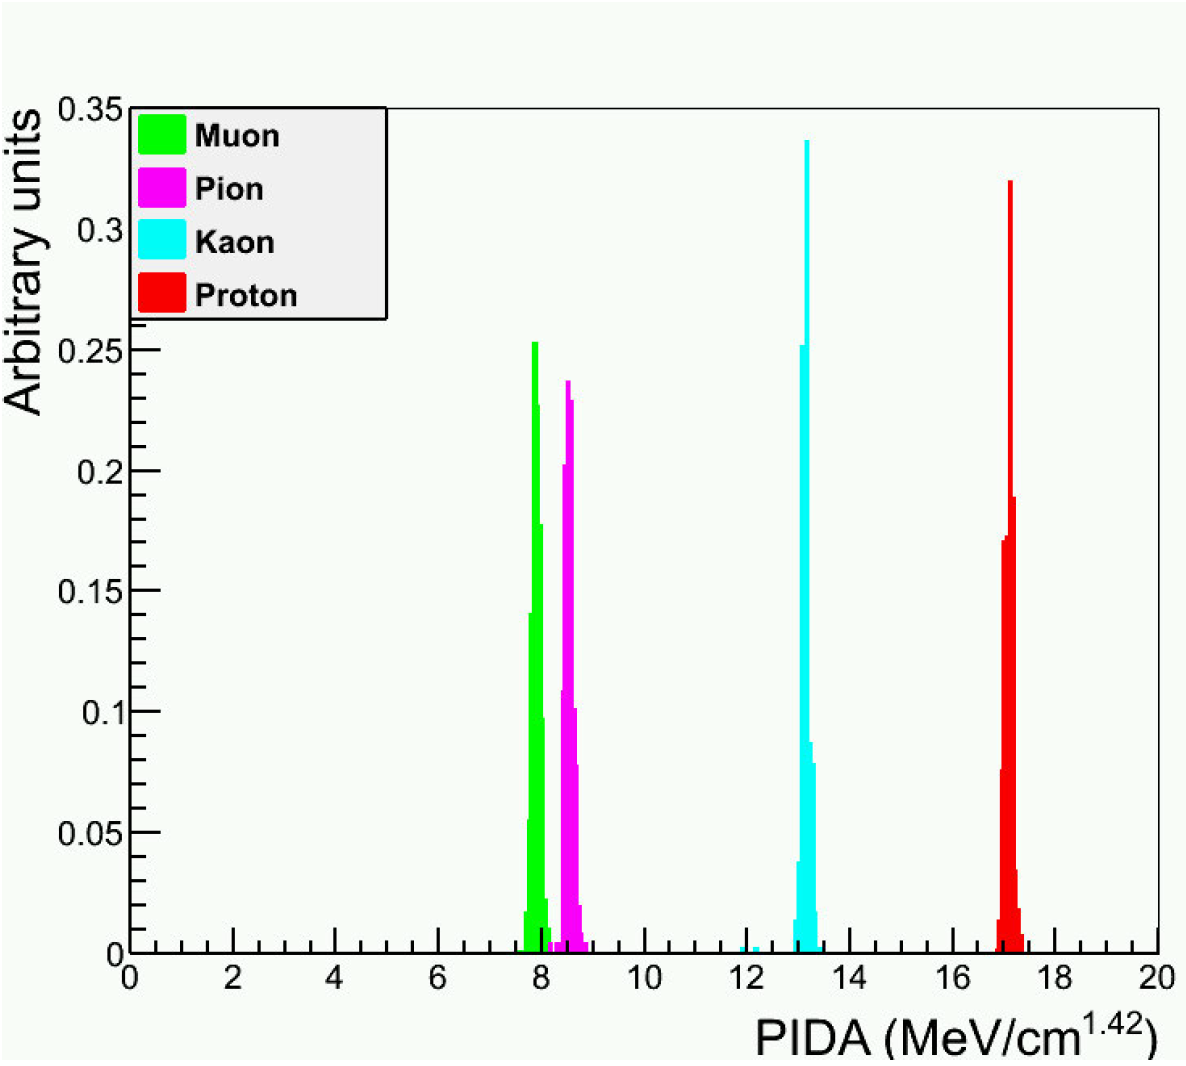
\includegraphics[width=0.5\textwidth]{TruthPIDA}
  \caption[The distribution of PIDA values, calculated using Monte Carlo truth, for different particle masses]
          {The distribution of PIDA values, calculated using Monte Carlo truth, for different particle masses. The figure is taken from~\citep{PIDA_Paper}.}
  \label{fig:PIDA_MC}
\end{figure}

From Figure~\ref{fig:PIDA_MC}, it can be seen that the most distinct PIDA distributions are that of muons and protons, these are also two of the most common charges particles in cosmic rays. For these reasons, particle identification using the PIDA variable, will be attempted in simulations of the 35 ton detector. As outlined in Sections~\ref{sec:SimInteractionTimes} and~\ref{sec:MCCalib}, in order to do this the interaction times of particles have to be well known, and the calibration constants must be tuned, so as to ensure that the effects of recombination are properly accounted for. It is also useful to use the information found in Section~\ref{sec:SimRecoEffic} about the efficiency with which tracks are reconstructed. In this regard, it is useful to produce additional figures showing the reconstruction efficiencies of protons in the CRY sample (Figure~\ref{fig:Prot_Effic}).\\

\begin{figure}
  \centering
  \begin{subfigure}{0.48\textwidth}
        \centering
        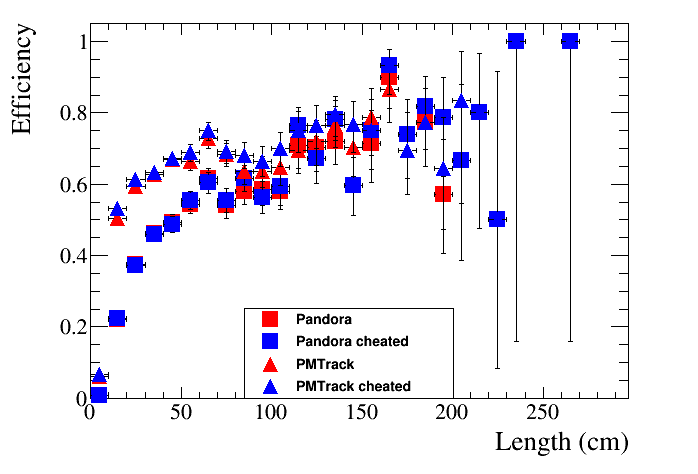
\includegraphics[width=\textwidth]{Effic_ProtonEnrich_500V_Proton_Length}
        \caption{The reconstruction efficiency as a function of the track length in the detector from Monte Carlo truth.}
        \label{fig:Prot_Effic_Len}
  \end{subfigure}%
  \hspace{0.03\textwidth}%
  \begin{subfigure}{0.48\textwidth}
        \centering
        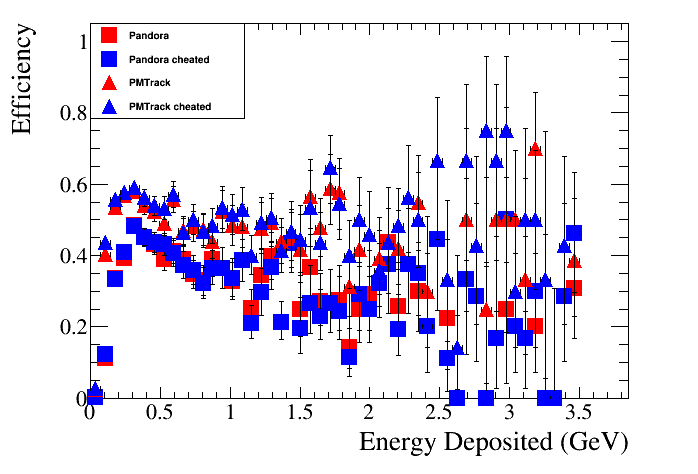
\includegraphics[width=\textwidth]{Effic_ProtonEnrich_500V_Proton_EnDepos}
        \caption{The reconstruction efficiency as a function of the deposited energy in the detector from Monte Carlo truth.}
        \label{fig:Prot_Effic_EnDepos}
  \end{subfigure}
  \begin{subfigure}{0.48\textwidth}
        \centering
        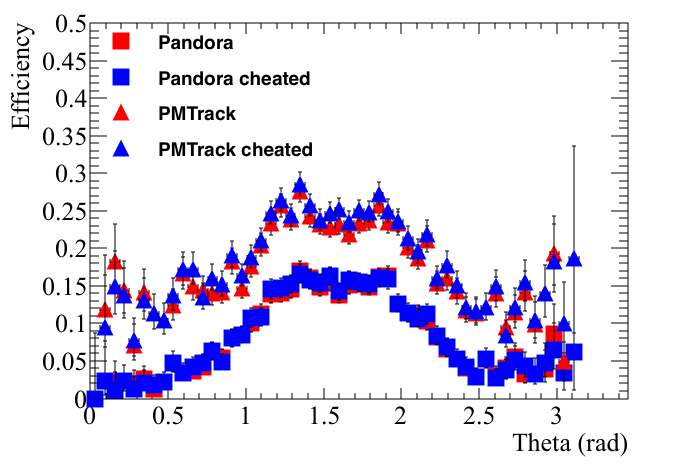
\includegraphics[width=\textwidth]{Effic_ProtonEnrich_500V_Proton_Theta}
        \caption{The reconstruction efficiency as a function of the $\theta$ track angle from Monte Carlo truth.}
        \label{fig:Prot_Effic_Theta}
  \end{subfigure}%
  \hspace{0.03\textwidth}%
  \begin{subfigure}{0.48\textwidth}
        \centering
        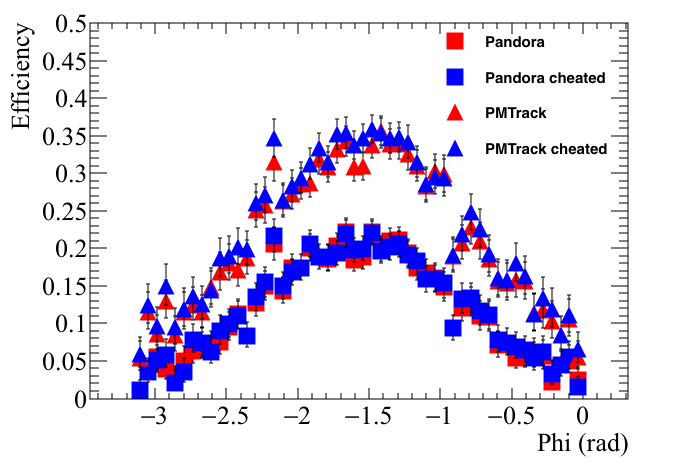
\includegraphics[width=\textwidth]{Effic_ProtonEnrich_500V_Proton_Phi}
        \caption{The reconstruction efficiency as a function of the $\phi$ track angle from Monte Carlo truth.}
        \label{fig:Prot_Effic_Phi}
  \end{subfigure}
%  \begin{subfigure}{0.8\textwidth}
%        \centering
%        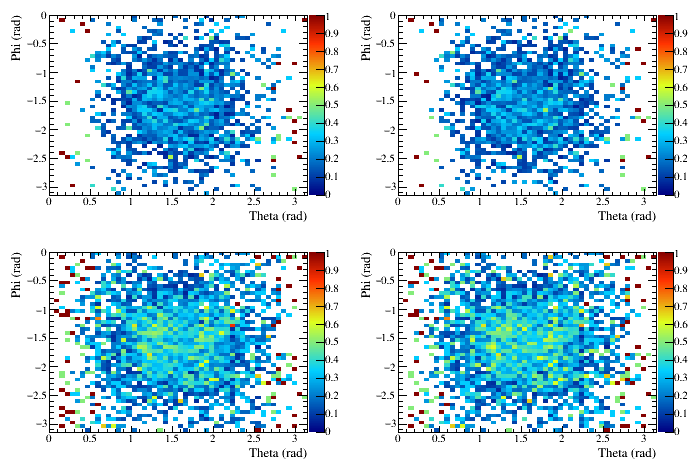
\includegraphics[width=\textwidth]{Effic_ProtonEnrich_500V_Proton_PhiTheta}
%        \caption{The reconstruction efficiency as a function of Monte Carlo truth track angle in $\theta$ and $\phi$. The track angle in $\theta$ is shown on the $x$ axis, and the track angle in $\phi$ is shown on the $y$ axis. The colour $z$ axis shows the reconstruction efficency.}
%        \label{fig:Prot_Effic_PhiTheta}
%  \end{subfigure}%
  \caption[The reconstruction efficiencies for protons in a sample generated using CRY.]
          {The reconstruction efficiencies for protons in a sample generated using CRY. Top left: the efficiencies as a function of the track length in the detector from Monte Carlo truth. Top right: the efficiencies as a function of the deposited energy from Monte Carlo truth. Bottom left: the efficiencies as a function of the $\theta$ track angle from Monte Carlo truth. Bottom right: the efficiencies as a function of the $\phi$ track angle from Monte Carlo truth. The efficiencies are shown for ``non-cheated'' reconstruction (red), and ``cheated'' reconstruction (blue), for both Pandora~\citep{Pandora} (squares) and PMTrack~\citep{PMTrack} (triangles).}
  \label{fig:Prot_Effic}
\end{figure}

Figure~\ref{fig:Prot_Effic} shows that the average reconstruction efficiency for PMTrack is higher than that for Pandora when considering protons. This can be easily seen in Figure~\ref{fig:Prot_Effic_Theta}, where the efficiency for PMTrack is roughly 10\% higher than that of Pandora, for all values of $\theta$. The reconstruction efficiency is still much lower than the overall efficiency shown in Figure~\ref{fig:SimEffic_Theta}, for both the positive muon and CRY samples though. This shows that the overall reconstruction efficiency for protons is quite low. Comparing Figures~\ref{fig:SimEffic_Length_CRY}, and~\ref{fig:Prot_Effic_Len}, it is evident that the reconstruction efficiency for protons with track lengths of more than 10~cm is reasonably similar to that of the overall reconstruction efficiency for the CRY sample, when using PMTrack. However, the reconstruction efficiency is significantly lower for protons with tracks of less than 10~cm. When using Pandora to reconstruct protons, the reconstruction efficiency is lower for all track lengths. It is found that 60\% of simulated protons have track lengths of less than 1~cm, and that none of these particles are reconstructed. It is this large number of very short particles which causes the overall reconstruction efficiency to be relatively low. When particles with track lengths of less than 1~cm (10~cm) are removed, the average reconstruction efficiency for PMTrack rises to 37\% (58\%). This shows that, when the shortest tracks are not counted, the reconstruction performs reasonably well. \\

It is also useful to produce samples where the primary particle is a single muon, or proton, located in the active volume of the detector. This allows for a sample of isolated tracks to be made, upon which the capabilities of the PIDA metric can be tested. It also allows the reconstruction efficiency to be found for particles in isolation. The properties of the generated particles are illustrated in Table~\ref{tab:IsolProp}. The values of the simulated quantities were found by changing the given parameters by an amount taken from a random sampling of a Gaussian distribution of width equal to the error listed. These simulation parameters were chosen to produce samples which would contain both exiting, and stopping particles, whilst generating the particles in the LAr would ensure that there should always be a reconstructable track in the detector. The reconstruction efficiencies when using the PMTrack reconstruction method are shown for the simulated particles in Figure~\ref{fig:Isol_Effic}. \\


Particles with track lengths of less than 1~cm have been excluded from these plots, which is why the angular reconstruction efficiencies for protons in Figures~\ref{fig:Isol_Effic_Theta} and~\ref{fig:Isol_Effic_Phi}, are higher than those seen in Figures~\ref{fig:Prot_Effic_Theta} and~\ref{fig:Prot_Effic_Phi}. This was done as none of these particles were reconstructed, due to the very short distances which they travel. After discounting these very short particles, the efficiencies generally follow similar patterns observed in the earlier efficiency plots, though there is a decrease in efficiencies for the longest track lengths which is not observed in other samples. This is attributed to the initial positions of the particles being within the detector volume, as this means that any particle travelling over 100~cm would have a very peculiar trajectory, as the edge of the detector should never be more than 100~cm away from the starting position. The only exception to this, is if a particle travelled along the $x$ axis to the other end of the detector. As discussed earlier, this is a very problematic orientation to reconstruct, as all of the charge would be deposited over a large range of time, on very few collection plane wires. \\

\begin{table}
\caption{The properties of initial particles simulated in the muon and proton samples. The angle $\theta_{xz}$, is defined as the angle that a vector makes in the $xz$ plane along the $x$ axis. The angle $\theta_{yz}$, is defined as the angle that a vector make in the $yz$ plane along the $z$ axis.}
\centering
\label{tab:IsolProp}
\begin{tabular}{l c c}
\toprule
{} & {Muon properties} & {Proton properties} \\ 
\midrule
Initial position (cm)              & (100 $\pm$ 50, 0 $\pm$ 30, 80 $\pm$ 20) & (100 $\pm$ 50, 0 $\pm$ 30, 80 $\pm$ 20)  \\

Initial momentum (GeV)            & 0.3 $\pm$ 0.1 & 0.8 $\pm$ 0.5 \\

Initial $\theta_{xz}$ $(^{\circ})$ &   0 $\pm$ 180 &   0 $\pm$ 180 \\

Initial $\theta_{yz}$ $(^{\circ})$ & -45 $\pm$ 45  & -45 $\pm$ 45  \\
\bottomrule
\end{tabular}
\end{table}

\begin{figure}
  \centering
  \begin{subfigure}{0.48\textwidth}
        \centering
        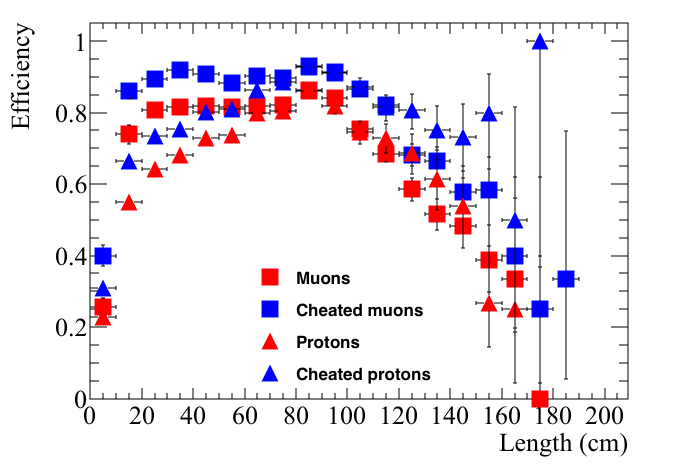
\includegraphics[width=\textwidth]{Effic_SingSamps_Length}
        \caption{The reconstruction efficiency as a function of the track length in the detector from Monte Carlo.}
        \label{fig:Isol_Effic_Len}
  \end{subfigure}%
  \hspace{0.03\textwidth}%
  \begin{subfigure}{0.48\textwidth}
        \centering
        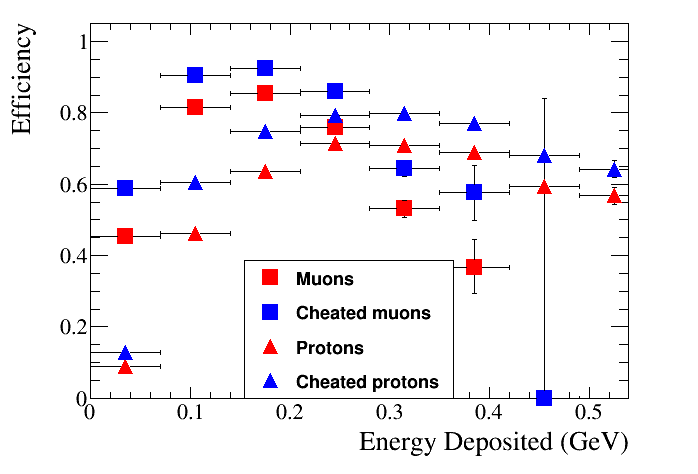
\includegraphics[width=\textwidth]{Effic_SingSamps_EnDepos}
        \caption{The reconstruction efficiency as a function of the deposited energy in the detector from Monte Carlo truth.}
        \label{fig:Isol_Effic_EnDepos}
  \end{subfigure}
  \begin{subfigure}{0.48\textwidth}
        \centering
        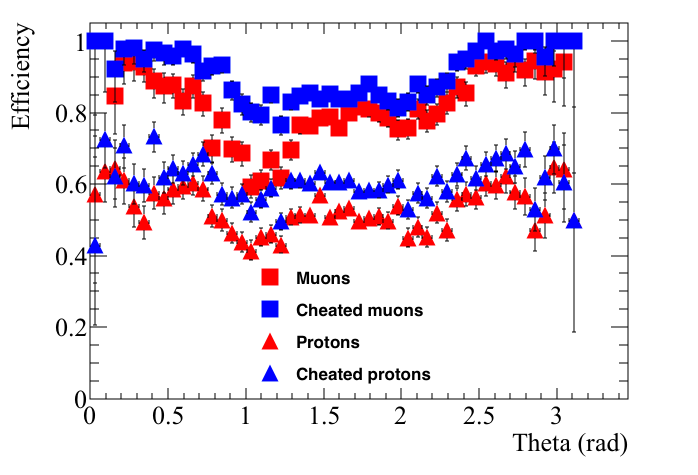
\includegraphics[width=\textwidth]{Effic_SingSamps_Theta}
        \caption{The reconstruction efficiency as a function of the $\theta$ track angle from Monte Carlo truth.}
        \label{fig:Isol_Effic_Theta}
  \end{subfigure}%
  \hspace{0.03\textwidth}%
  \begin{subfigure}{0.48\textwidth}
        \centering
        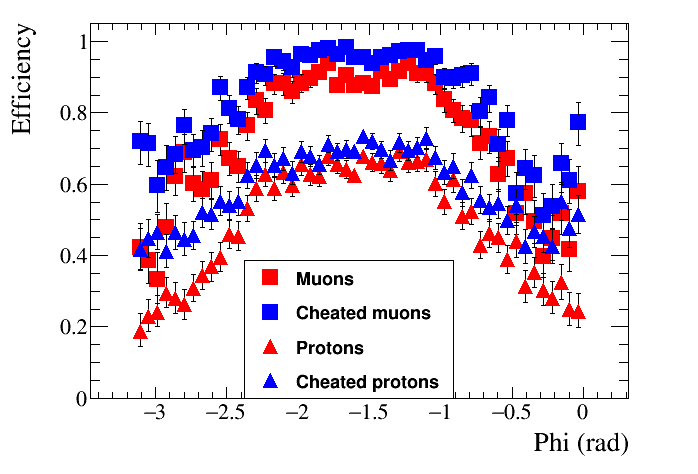
\includegraphics[width=\textwidth]{Effic_SingSamps_Phi}
        \caption{The reconstruction efficiency as a function of the $\phi$ track angle from Monte Carlo truth.}
        \label{fig:Isol_Effic_Phi}
  \end{subfigure}
%  \begin{subfigure}{0.8\textwidth}
%        \centering
%        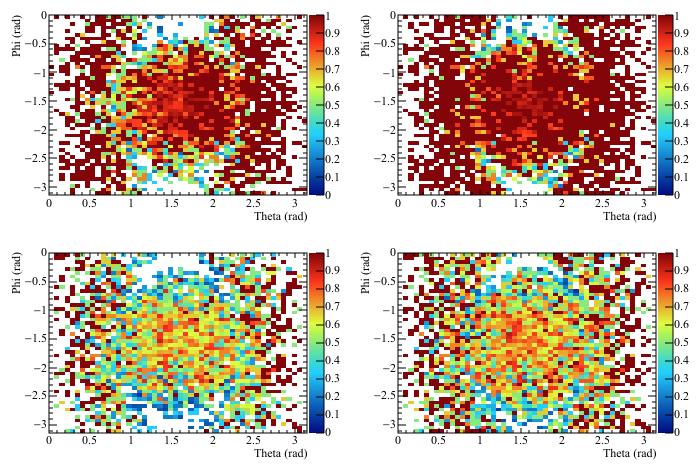
\includegraphics[width=\textwidth]{Effic_SingSamps_PhiTheta}
%        \caption{The reconstruction efficiency as a function of Monte Carlo truth track angle in $\theta$ and $\phi$. The track angle in $\theta$ is shown on the $x$ axis, and the track angle in $\phi$ is shown on the $y$ axis. The colour $z$ axis shows the reconstruction efficency.}
%        \label{fig:Isol_Effic_PhiTheta}
%  \end{subfigure}%
  \caption[The reconstruction efficiencies for the simulated isolated muon and proton samples in the 35 ton detector.]
          {The reconstruction efficiencies for the simulated isolated muon and proton samples in the 35 ton detector. Top left: the efficiencies as a function of the track length in the detector from Monte Carlo truth. Top right: the efficiencies as a function of the deposited energy from Monte Carlo truth. Bottom left: the efficiencies as a function of the $\theta$ track angle from Monte Carlo truth. Bottom right: the efficiencies as a function of the $\phi$ track angle from Monte Carlo truth. The efficiencies are shown for 'non-cheated' reconstruction (red), and 'cheated' reconstruction (blue), for both Pandora~\citep{Pandora} (squares) and PMTrack~\citep{PMTrack} (triangles).}
   \label{fig:Isol_Effic}
\end{figure}

As the increase in $\frac{dE}{dx}$ is only visible when the particle stops in the detector, it is necessary to remove exiting particles from the sample. This is done by applying a fiducial cut on the end point of the reconstructed track. It is important to only place this on the end point of the track, as one does not want to remove particles which enter the detector and then stop. When calorimetry is performed, the end point of the track is determined using, among other metrics, the increase in $\frac{dE}{dx}$, and so the residual range of the track (a stored data member of the track object), and so should always refer to the distance to the end of the particles trajectory. For this study, a fiducial cut of 5~cm is used. This means that any track with hits within 5~cm of the edge of the detector volume is discarded, and counted as an exiting particle. This should mean that very few tracks due to exiting particles are identified as stopping in the detector, as it would require the reconstruction algorithms to miss a large section of the track. This will mean that some stopping particles are incorrectly assigned as exiting particles, causing the identification efficiency to drop, but it is necessary to ensure that exiting particles are not included in the final distributions. A further cut that is applied, is the requirement that the track contains a minimum of 10 collection plane hits, this is to ensure that an adequate number of points are taken upon which to find an average value of PIDA for the track. Similar cuts are described in~\citep{PIDA_Paper}, and the resulting distributions of PIDA values for the isolated muon, and isolated proton samples, are shown in Figure~\ref{fig:Isol_PIDA}. \\

\begin{figure}
  \centering
  \begin{subfigure}{0.6\textwidth}
        \centering
        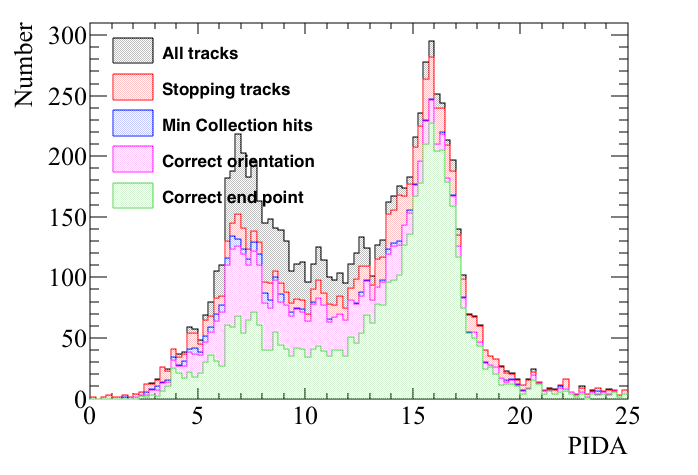
\includegraphics[width=\textwidth]{IsolatedProtons_500V_Dec16_Proton_PIDA}
        \caption{The PIDA values calculated for the isolated proton sample.}
        \label{fig:Isol_PIDA_Proton}
  \end{subfigure}
  \begin{subfigure}{0.6\textwidth}
        \centering
        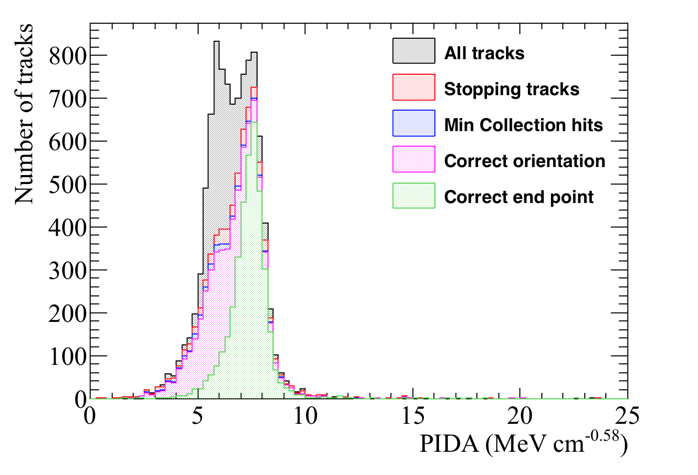
\includegraphics[width=\textwidth]{IsolatedMuons_500V_Dec16_Muon_PIDA}
        \caption{The PIDA values calculated for the isolated muon sample.}
        \label{fig:Isol_PIDA_Muon}
  \end{subfigure}
  \caption[The calculated PIDA values for the simulated isolated proton and muon samples in the 35 ton detector.]
          {The calculated PIDA values for the simulated isolated proton (top) and muon (bottom) samples in the 35 ton detector. A series of criteria designed to select only tracks due to stopping particles which have a required number of collection plane hits is applied. The tracks are then further refined using truth information such as the true end point of the particle.}
  \label{fig:Isol_PIDA}
\end{figure}

As can be seen from Figure~\ref{fig:Isol_PIDA}, using Monte Carlo truth information can make the distributions much cleaner, particularly when discounting particles for which the reconstruction algorithms do not track to their end point. A track is identified as having a correctly reconstructed end point, if the reconstructed end point is within 2.5~cm of the end point of the particle from Monte Carlo truth. It is reassuring to see that few tracks are reconstructed backwards, as if this were not the case then performing particle identification would be very difficult. This is because, it would indicate that the calorimetry and tracking algorithms are not performing well. However, improvements can still be made, as both plots in Figure~\ref{fig:Isol_PIDA} contain many tracks which do not extend to the end points of the particles from Monte Carlo truth. This can be seen as when the requirement that the reconstructed track end point is consistent with the end point from Monte Carlo truth, the low tails of the PIDA distributions are significantly reduced. This is most noticeably the case in Figure~\ref{fig:Isol_PIDA_Muon}, where the peak at low values of PIDA is significantly reduced. It is observed that the PIDA distributions are cleaner when information from all three wire planes are used, as opposed to only using the collection plane, and so this is presented here. This shows how important it is to calibrate the electronics responses of all three wire planes, and how additional wire planes can improve calorimetry, as well as the accuracy of reconstruction algorithms~\citep{XinSeptFNAL}. \\

Figure~\ref{fig:Isol_dEdx} shows the relationship between the $\frac{dE}{dx}$ and residual range of a track, for both protons and muons. The much steeper increase in $\frac{dE}{dx}$ at low residual ranges for protons, compared to muons, is clearly visible when comparing Figures~\ref{fig:Isol_dEdx_Proton} and~\ref{fig:Isol_dEdx_Muon}. The contamination in the proton sample at low PIDA can be seen in Figure~\ref{fig:Isol_dEdx_Proton}, where there is a clear sample of tracks for which the $\frac{dE}{dx}$ does not increase for low residual ranges. These plots are filled after tracks whose end points do not correlate with the end points from Monte Carlo truth are removed, and so the tail of low $\frac{dE}{dx}$ values is due to particles for which the simulated detector did not find increased energy depositions as the particle stopped. It is therefore possible that at least some of these protons do not in fact stop, but interact inelastically when they still have a significant amount of kinetic energy. When this occurs, GEANT4 and the tracking algorithms, will create a new particle or track, which would be tracked to the true end point of the particle. However, the ``end-point'' of the initial particle will be before the particle actually stopped, and so it will have a MIP-like distribution in Figure~\ref{fig:Isol_dEdx_Proton}. \\

\begin{figure}
  \centering
  \begin{subfigure}{0.48\textwidth}
        \centering
        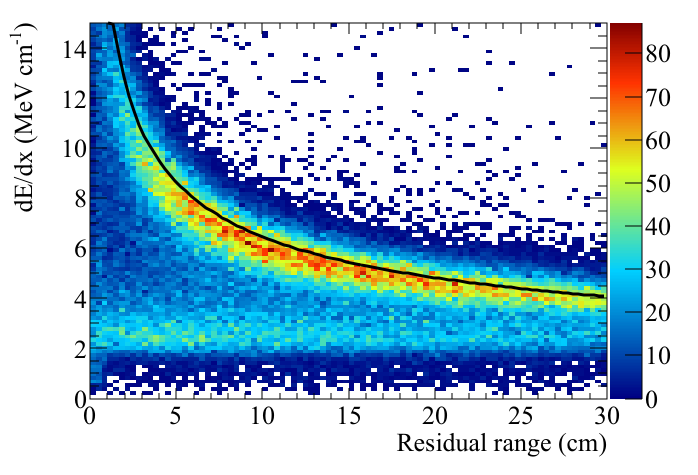
\includegraphics[width=\textwidth]{IsolatedProtons_500V_Dec16_Proton_dEdx}
        \caption{The $\frac{dE}{dx}$ versus residual range plot for the simulated isolated proton sample.}
        \label{fig:Isol_dEdx_Proton}
  \end{subfigure}%
  \hspace{0.03\textwidth}%
  \begin{subfigure}{0.48\textwidth}
        \centering
        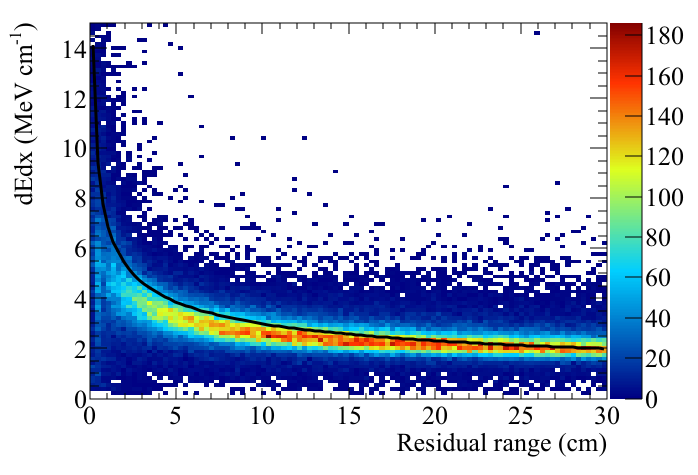
\includegraphics[width=\textwidth]{IsolatedMuons_500V_Dec16_Muon_dEdx}
        \caption{The $\frac{dE}{dx}$ versus residual range plot for the simulated isolated muon sample.}
        \label{fig:Isol_dEdx_Muon}
  \end{subfigure}
  \caption[The $\frac{dE}{dx}$ versus residual range plot for the simulated isolated proton and muon samples in the 35 ton detector.]
          {The measured relationship between $\frac{dE}{dx}$ and residual range for the simulated isolated proton (left) and muon (right) samples in the 35 ton detector. The balck curves show the parameterisation given by the Bethe-Block equation (Equation~\ref{eq:Bethe-Bloch} for each particle species. These plots are made after applying all of the cuts outlined in Figure~\ref{fig:Isol_PIDA}, meaning that only hits from tracks whose end points are consistent with the end points from Monte Carlo truth are plotted.}
  \label{fig:Isol_dEdx}
\end{figure}

%\begin{figure}
%  \centering
%  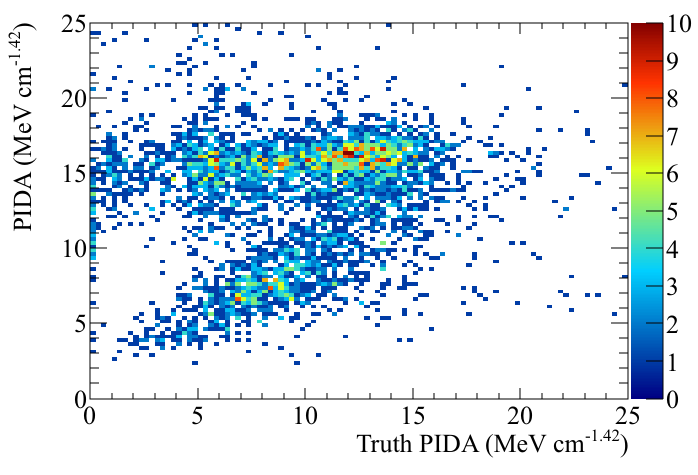
\includegraphics[width=0.5\textwidth]{IsolatedProtons_500V_Dec16_Proton_MCPIDA_PIDA}
%  \caption[A comparison between PIDA values calculated using truth and reconstructed information]
%          {A comparison between PIDA values calculated using truth and reconstructed information}
%  \label{fig:MCPIDA}
%\end{figure}

It is useful to summarise the information shown in Figure~\ref{fig:Isol_PIDA} in a table, so that an efficiency of identifying stopping particles can be found. This is shown in Table~\ref{tab:Isol_PIDA_Proton} for protons, and in Table~\ref{tab:Isol_PIDA_Muon} for muons. The efficiency shown in these tables is defined as the number of tracks in the PIDA range, divided by the total number of stopping particles. This means that it is possible to have an efficiency of more than 100\%, if more reconstructed tracks have PIDA values within the PIDA range than there are stopping particles from Monte Carlo truth. This is the case in Table~\ref{tab:Isol_PIDA_Muon}, where there are initially more reconstructed tracks than stopping particles within the PIDA range. The purity shown in these tables is defined as the percentage of tracks in the PIDA range associated with particles that stop in the detector from Monte Carlo truth. As many of the tracks shown in the ``reconstructed tracks'' row in Table~\ref{tab:Isol_PIDA_Muon} are not due to stopping particles, the initial purity is low, though this increases markedly after the fiducial cut is applied. The PIDA ranges referred to are 14-18~MeV$\cdot$cm$^{-1.42}$, and 5-9~MeV$\cdot$cm$^{-1.42}$, for protons and muons respectively, as these ranges cover the peaks of the distributions shown in Figure~\ref{fig:Isol_dEdx}, and are centred on the peaks in Figure~\ref{fig:PIDA_MC}. \\

As can be seen in Table~\ref{tab:Isol_PIDA_Proton}, the efficiency upon which protons can be identified does not change significantly as the sequential criteria are applied, but, as shown in Figure~\ref{fig:Isol_PIDA_Proton}, the peak at low values of PIDA decreases significantly. The same cannot be said for the muon sample however, as when the criteria that the tracking end point matches the end point from Monte Carlo truth is applied, a significant section of the tail within the PIDA range is removed, significantly reducing the PIDA efficiency. However, the resulting distribution is more similar to that shown in Figure~\ref{fig:PIDA_MC}, showing that the particles which survive the cut are those that are very well reconstructed. The cut to remove tracks that do not have the correct end points from Monte Carlo truth reduces both sets of efficiencies, but, if all particles were reconstructed with the correct end points, then one can imagine that the number of tracks within the PIDA ranges would increase, and the distributions would become more symmetrical, as shown in Figure~\ref{fig:Isol_PIDA_Muon}. Both tables also exhibit high purities, which shows that the fiducial cut, designed to removing exiting particles, is effective, with only 2 exiting protons being mis-identified in the proton sample. \\

\begin{table}
  \caption[A summary of the PIDA values calculated for the simulated isolated proton sample, as sequential cuts are applied]
          {A summary of the PIDA values calculated for the simulated isolated proton sample, as sequential cuts are applied.}
  \centering
  \label{tab:Isol_PIDA_Proton}
  \begin{tabular}{l c c c c}
    \toprule
    \multirow{2}{*}{Applied cut} & \multicolumn{3}{c}{Proton sample} \\ 
    \cmidrule{2-5}
      & Tracks & In PIDA range & Efficiency & Purity \\ 
    \midrule
      Total stopping particles            & 13295 &     &        & \\

      Reconstructed tracks                & 8761 & 3009 & 22.6\% & 98.7\% \\

      Survives 5~cm fiducial cut          & 7552 & 2894 & 21.8\% & 99.9\% \\

      Minimum of 10 collection plane hits & 6186 & 2507 & 18.9\% & 99.9\% \\

      Correct track orientation           & 6022 & 2491 & 18.7\% & 99.9\% \\

      Correct tracking end point          & 4588 & 2327 & 17.5\% & 100\% \\
    \bottomrule
  \end{tabular}
\end{table}

\begin{table}
  \caption[A summary of the PIDA values calculated for the simulated isolated muon sample, as sequential cuts are applied]
          {A summary of the PIDA values calculated for the simulated isolated muon sample, as sequential cuts are applied.}
  \centering
  \label{tab:Isol_PIDA_Muon}
  \begin{tabular}{l c c c c}
    \toprule
    \multirow{2}{*}{Applied cut} & \multicolumn{3}{c}{Muon sample} \\ 
    \cmidrule{2-5}
      & Tracks & In PIDA range & Efficiency & Purity \\ 
    \midrule
      Total stopping particles            & 6880 &      &        & \\

      Reconstructed tracks                & 9883 & 8907 & 129\%  & 67.4\% \\

      Survives 5~cm fiducial cut          & 7126 & 6259 & 90.9\% & 90.2\% \\

      Minimum of 10 collection plane hits & 6580 & 5876 & 85.4\% & 89.9\% \\

      Correct track orientation           & 6436 & 5767 & 83.8\% & 90.1\% \\

      Correct tracking end point          & 3832 & 3699 & 53.8\% & 100\%  \\
    \bottomrule
  \end{tabular}
\end{table}

From Table~\ref{tab:Isol_PIDA_Proton}, it can be seen that there are more stopping protons than primary protons, as only 10,000 primary protons were generated. The effectiveness of the PIDA algorithm at identifying only primary protons is shown in Table~\ref{tab:Isol_PIDA_PrimProton}. Comparing both tables, it can be seen that the efficiency with which the primary protons can be identified is larger than the secondary protons, as the efficiencies shown in Table~\ref{tab:Isol_PIDA_Proton} are lower than those in Table~\ref{tab:Isol_PIDA_PrimProton}. It is thought that this is due to the low reconstruction efficiency for particles with the shortest track lengths, as many of the secondary protons will have short track lengths in the detector from Monte Carlo truth, as discussed in Section~\ref{sec:SimRecoEffic}. A similar table is not produced for primary muons, as there were no secondary muons produced in the isolated muon sample, and so Table~\ref{tab:Isol_PIDA_Muon} is itself the efficiency with which the primary muons can be identified. \\ 

\begin{table}
  \caption[A summary of the PIDA values calculated for the primary particles in the simulated isolated proton sample, as sequential cuts are applied]
          {A summary of the PIDA values calculated for the primary particles in the simulated isolated proton sample, as sequential cuts are applied.}
  \centering
  \label{tab:Isol_PIDA_PrimProton}
  \begin{tabular}{l c c c c}
    \toprule
    \multirow{2}{*}{Applied cut} & \multicolumn{3}{c}{Proton sample} \\ 
    \cmidrule{2-5}
      & Tracks & In PIDA range & Efficiency & Purity \\ 
    \midrule
      Total stopping particles            & 7798 &      &        & \\

      Reconstructed tracks                & 5920 & 1937 & 24.8\% & 98.9\% \\

      Survives 5~cm fiducial cut          & 5044 & 1878 & 24.1\% & 99.9\% \\

      Minimum of 10 collection plane hits & 4485 & 1711 & 21.9\% & 99.9\% \\

      Correct track orientation           & 4363 & 1707 & 21.9\% & 99.9\% \\

      Correct tracking end point          & 3246 & 1595 & 20.4\% & 100\%  \\
    \bottomrule
  \end{tabular}
\end{table}

Upon verifying that the PIDA metric can reliably determine particle type when they are simulated in isolation, the next step is to observe the accuracy with which particles can be identified in a CRY sample. The sample used here differs from the CRY sample used earlier, in that only events which contain a proton track in the detector from Monte Carlo truth are reconstructed. This is done to reduce simulation time and storage space, as this cut will still provide a substantial number of muons, whilst ensuring that a large proton sample can be reconstructed. This sample is thus called the ``proton enriched CRY sample'.'' \\

The process of calculating PIDA values for tracks is identical in all samples, though, as discussed in Section~\ref{sec:SimRecoEffic}, the much more complicated event structure in the CRY sample affects the reconstruction efficiency, and so will likely also affect the accuracy of the calorimetry. The calorimetry will be affected in two ways, firstly, the reduced performance of the reconstruction algorithms will mean that some particles are not reconstructed at all, whilst those that are reconstructed may be more likely to have missing hits, and so the end points may be reconstructed less accurately. This will cause the tail of low $\frac{dE}{dx}$ values, seen in Figure~\ref{fig:Isol_dEdx_Proton}, to be more pronounced. Secondly, though the photon detector time determination is very accurate for a large number of tracks, it is also incorrect for a number of tracks, as shown in Figure~\ref{fig:PD_MCPDDiff}. This will cause the $x$ position correction to be miscalculated, which will in turn increase the calculated $\frac{dE}{dx}$, and hence PIDA values. For this reason, it is also useful to present the PID efficiency when using cheated reconstruction, so that the effect of incorrectly determining the interaction time, and performing incorrect disambiguation, can be seen. \\

The PIDA values calculated for protons and muons in the proton enriched CRY sample are shown in Figure~\ref{fig:CRY_PIDA}. The PIDA distributions when the reconstruction is both ``cheated,'' and not ``cheated'' are shown. \\

%%%%%%% The raw PIDA plots......
\begin{figure}
  \centering
  \begin{subfigure}{0.48\textwidth}
        \centering
        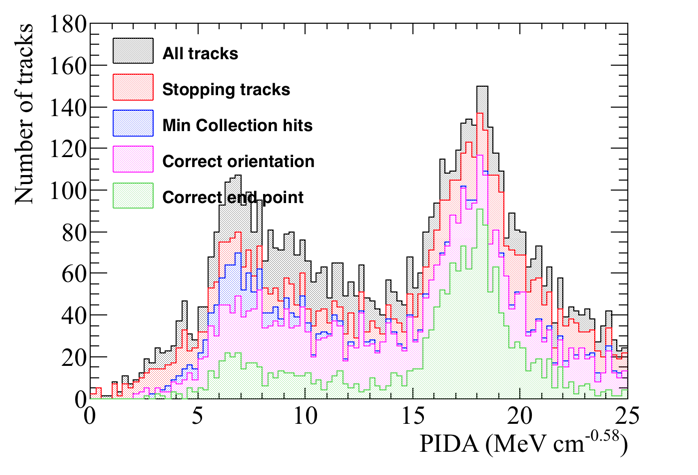
\includegraphics[width=\textwidth]{ProtonEnrich_500V_v05_14_00_trackpmtrackT0_Proton_PIDA}
        \caption{The PIDA values calculated for protons, using the photon detectors to calculate an interaction time.}
        \label{fig:CRY_PIDA_Proton_NonCheat}
  \end{subfigure}%
  \hspace{0.03\textwidth}%
  \begin{subfigure}{0.48\textwidth}
        \centering
        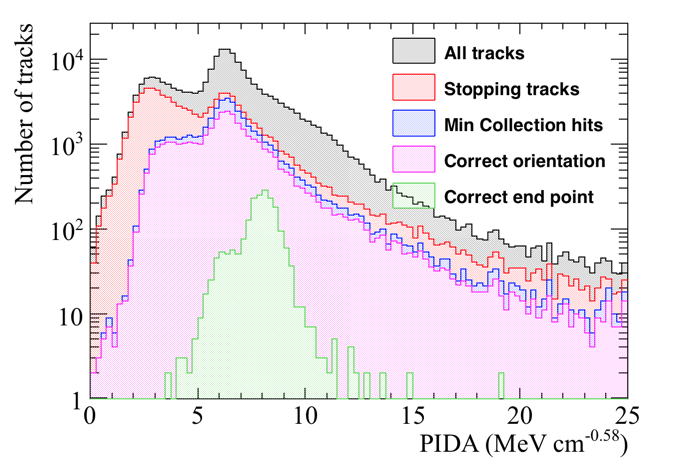
\includegraphics[width=\textwidth]{ProtonEnrich_500V_v05_14_00_trackpmtrackT0_Muon_PIDA}
        \caption{The PIDA values calculated for muons, using the photon detectors to calculate an interaction time.}
        \label{fig:CRY_PIDA_Muon_NonCheat}
  \end{subfigure}
  %%%%%%%%%%%
  \begin{subfigure}{0.48\textwidth}
        \centering
        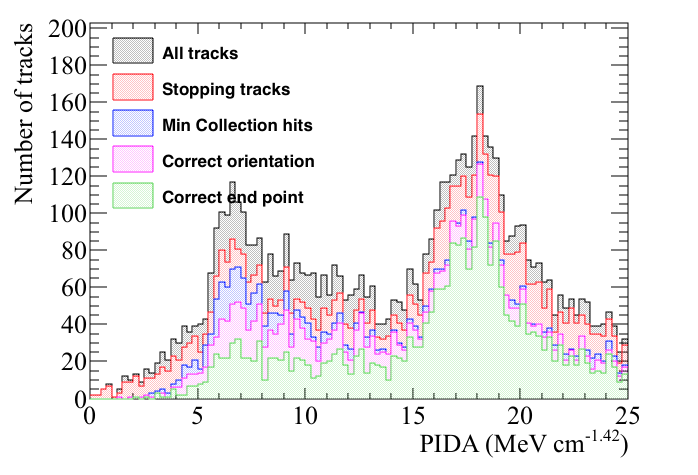
\includegraphics[width=\textwidth]{ProtonEnrich_500V_v05_14_00_trackpmtrackdc_Proton_PIDA}
        \caption{The PIDA values calculated for protons, using cheated reconstruction.}
        \label{fig:CRY_PIDA_Proton_Cheat}
  \end{subfigure}%
  \hspace{0.03\textwidth}%
  \begin{subfigure}{0.48\textwidth}
        \centering
        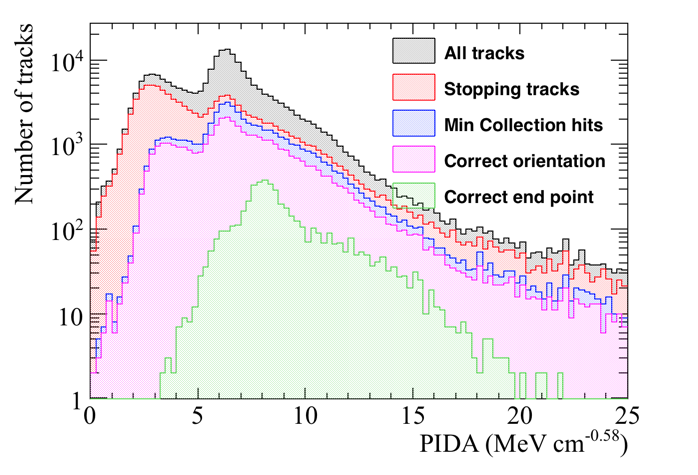
\includegraphics[width=\textwidth]{ProtonEnrich_500V_v05_14_00_trackpmtrackdc_Muon_PIDA}
        \caption{The PIDA values calculated for muons, using cheated reconstruction.}
        \label{fig:CRY_PIDA_Muon_Cheat}
  \end{subfigure}
  \caption[The calculated PIDA values for the simulated proton enriched sample in the 35 ton detector]
          {The calculated PIDA values for the simulated proton enriched sample in the 35 ton detector. Top left: the PIDA values calculated for protons using the photon detectors to measure the interaction time. Top right: the PIDA values calculated for muons using the photon detectors to measure the interaction time. Bottom left: PIDA values calculated for protons using a cheated interaction time determination. Bottom right: the PIDA values calculated for muons using a cheated interaction time determination. A series of criteria designed to select only tracks due to stopping particles which have a required number of collection plane hits is applied. The tracks are then further refined using truth information such as the true end point of the particle.}
  \label{fig:CRY_PIDA}
\end{figure}

From Figure~\ref{fig:CRY_PIDA}, it can be seen that the proton tracks which are reconstructed in the proton enriched sample, look very similar to the proton tracks which were reconstructed in the isolated proton sample, shown in Figure~\ref{fig:Isol_PIDA_Proton}. This is reassuring, as it shows that even when protons are surrounded by multiple cosmic rays, the reconstruction algorithms are still able to accurately reconstruct proton tracks. The benefit of performing ``cheated'' reconstruction can be seen by comparing Figures~\ref{fig:CRY_PIDA_Proton_NonCheat}, and~\ref{fig:CRY_PIDA_Proton_Cheat}, where the number of proton tracks that survive the application of all cuts is seen to increase. When the reconstruction is performed using non-cheated disambiguation, and a cheated interaction time determination, the distribution of events surviving the application of all cuts is seen to be very similar to Figure~\ref{fig:CRY_PIDA_Proton_Cheat}. This implies that the increase in the number of potentially identifiable proton tracks seen in Figure~\ref{fig:CRY_PIDA_Proton_Cheat}, is largely due to the increased accuracy of interaction time determination. \\

Though the plots shown in Figure~\ref{fig:CRY_PIDA} concerning the identification of protons are encouraging, the complementary plots concerning the identification of muons are much less encouraging. This is because, though there is quite a large peak at a PIDA value of around 8 MeV$\cdot$cm$^{-1}$ after the application of all cuts, this cannot be seen before the last cut is applied. This is because of two large peaks with PIDA values of around 3~MeV$\cdot$cm$^{-1}$ and 6~MeV$\cdot$cm$^{-1}$. A large peak at a PIDA value of 6 MeV$\cdot$cm$^{-1}$ was observed in Figure~\ref{fig:Isol_PIDA_Muon}, though this was largely removed by requiring that the muon track stopped in the detector. Unfortunately, this is not seen to be the case when considering muons in the enriched proton sample, though the size of the peak is significantly reduced by requiring that the track stops in the detector. Therefore, it is thought that the tracks which make up the peak of PIDA values at 6 MeV$\cdot$cm$^{-1}$, are partially reconstructed muon tracks. Effectively removing these partially reconstructed tracks is difficult, though if some degree of supplemental track stitching is performed during the analysis stage, they may be able to be removed. Evidence that this may work is presented in Figure~\ref{fig:CRY_PIDACheat}, where through-going particles from Monte Carlo truth have been removed. \\

A feature of Figures~\ref{fig:CRY_PIDA_Muon_NonCheat}, and~\ref{fig:CRY_PIDA_Muon_Cheat}, which was not present in Figure~\ref{fig:Isol_PIDA_Muon}, is the presence of a large peak at PIDA values of 3 MeV$\cdot$cm$^{-1}$. It is thought that this is due to very short delta rays coming off the high energy muon track as it passes through the detector. These tracks are considered to be due to the muon in the current framework, as the delta rays are not saved by GEANT4, and so LArSoft assigns any tracks which they produce to the parent of the electron, which in this case is the muon. Figures~\ref{fig:CRY_PIDATrLen_Muon_All},~\ref{fig:CRY_MCRecoRat_Muon_All}, and~\ref{fig:CRY_MCRecoTrack_Muon_All} support this assessment. From Figure~\ref{fig:CRY_PIDATrLen_Muon_All}, it can be seen that many of the tracks with very low values of PIDA have track lengths below 10~cm, which is much shorter than one would expect for a cosmic ray muon. This is conclusively shown by Figures~\ref{fig:CRY_MCRecoRat_Muon_All}, and~\ref{fig:CRY_MCRecoTrack_Muon_All}, as it can be seen that the muon tracks which have low PIDA values have very short reconstructed track lengths, compared to the track length in the detector from Monte Carlo truth. Figure~\ref{fig:CRY_MCRecoTrack_Muon_All}, then shows that many of the shortest reconstructed tracks, are associated with particles which have track lengths in the detector from Monte Carlo truth, which are much longer than themselves. Placing a cut at a minimum track length of 10~cm will also remove some of the muon tracks which contaminate the range of PIDA values expected for protons. However, it can be seen from Figures~\ref{fig:CRY_PIDATrLen_Proton_All}, and~\ref{fig:CRY_PIDATrLen_Proton_End}, that though some of the proton tracks which have PIDA values within the expected range will also be removed. It may therefore be necessary to develop a more sophisticated cut to remove these delta rays, should the identification of protons be attempted in the cosmic ray data collected by the 35 ton detector. Neither the development of such a cut, or the attempt to identify protons from cosmic ray data collected by the 35 ton detector, is presented here though. \\

%%%%%% The Reconstructed track length vs PIDA
\begin{figure}
  \centering
  \begin{subfigure}{0.48\textwidth}
        \centering
        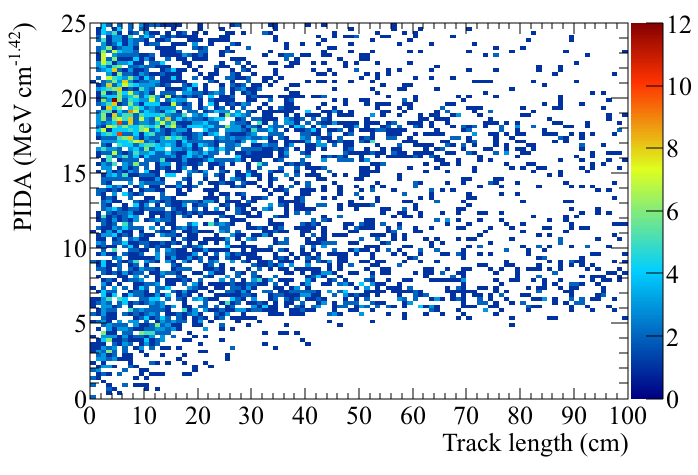
\includegraphics[width=\textwidth]{ProtonEnrich_500V_v05_14_00_trackpmtrackdc_Proton_All_PIDA_TrackLen}
        \caption{The calculated PIDA value for protons as a function of the reconstructed track length, filled for all tracks.}
        \label{fig:CRY_PIDATrLen_Proton_All}
  \end{subfigure}%
  \hspace{0.03\textwidth}%
  \begin{subfigure}{0.48\textwidth}
        \centering
        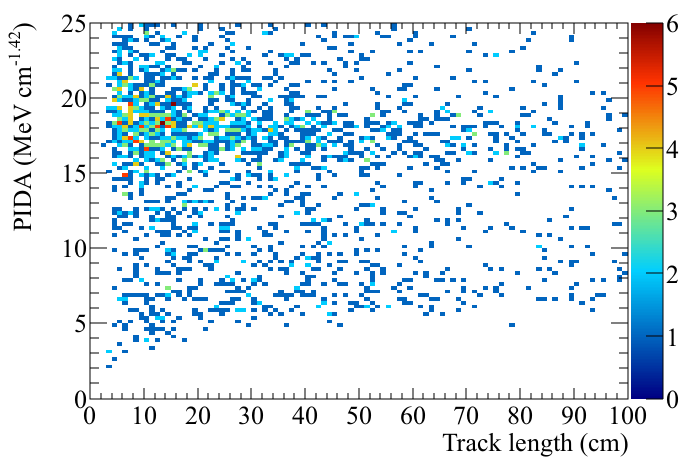
\includegraphics[width=\textwidth]{ProtonEnrich_500V_v05_14_00_trackpmtrackdc_Proton_End_PIDA_TrackLen}
        \caption{The calculated PIDA value for protons as a function of the reconstructed track length, filled for tracks which pass all cuts.}
        \label{fig:CRY_PIDATrLen_Proton_End}
  \end{subfigure}
  %%%%%%%%%%%
  \begin{subfigure}{0.48\textwidth}
        \centering
        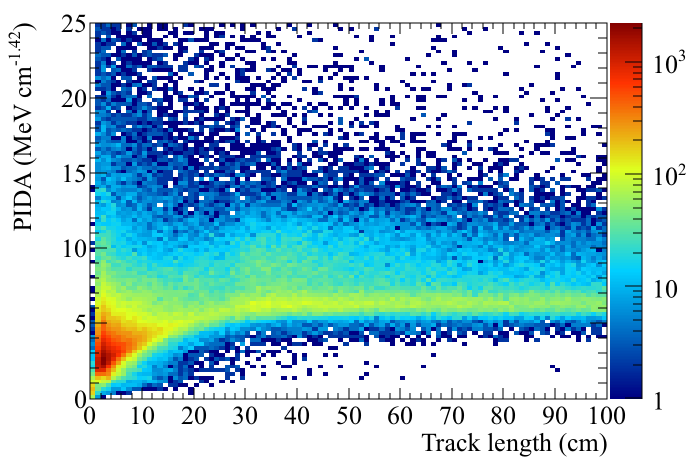
\includegraphics[width=\textwidth]{ProtonEnrich_500V_v05_14_00_trackpmtrackdc_Muon_All_PIDA_TrackLen}
        \caption{The calculated PIDA value for muons as a function of the reconstructed track length, filled for all tracks.}
        \label{fig:CRY_PIDATrLen_Muon_All}
  \end{subfigure}%
  \hspace{0.03\textwidth}%
  \begin{subfigure}{0.48\textwidth}
        \centering
        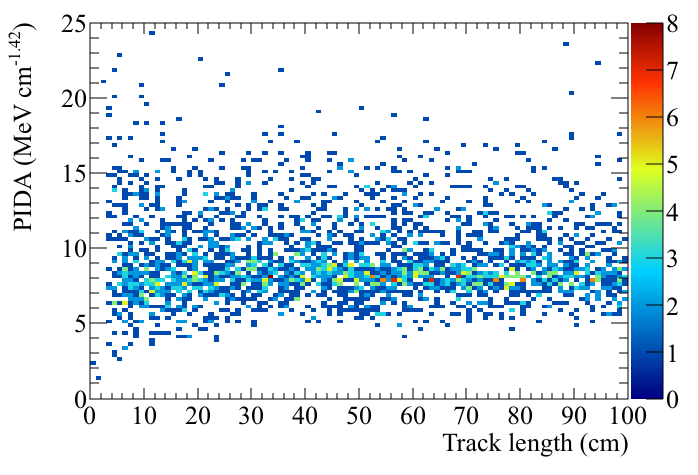
\includegraphics[width=\textwidth]{ProtonEnrich_500V_v05_14_00_trackpmtrackdc_Muon_End_PIDA_TrackLen}
        \caption{The calculated PIDA value for muons as a function of the reconstructed track length, filled for tracks which pass all cuts.}
        \label{fig:CRY_PIDATrLen_Muon_End}
  \end{subfigure}
  \caption[The calculated PIDA values, as a function of the reconstructed track length, for the simulated proton enriched sample in the 35 ton detector]
          {The calculated PIDA values, as a function of the reconstructed track length, for the simulated proton enriched sample in the 35 ton detector. Top left: the PIDA values, as a function of the reconstructed track length, when filled for all proton tracks. Top right: the PIDA values, as a function of the reconstructed track, filled for proton tracks which pass all cuts. Bottom left: the PIDA values, as a function of the reconstructed track length, when filled for all muon tracks. Top right: the PIDA values, as a function of the reconstructed track, filled for muon tracks which pass all cuts. All plots are made for tracks which have been reconstructed using a cheated interaction time determination.}
  \label{fig:CRY_PIDATrLen_PIDA}
\end{figure}

%%%%%% The ratio of reco track length vs PIDA, and reco vs true track length
\begin{figure}
  \centering
  \begin{subfigure}{0.48\textwidth}
        \centering
        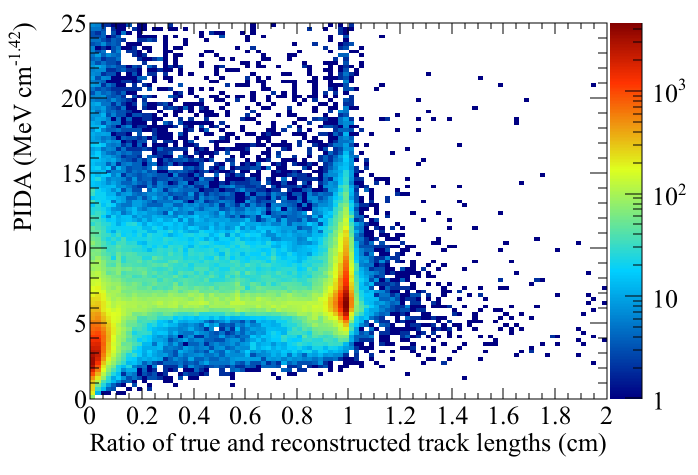
\includegraphics[width=\textwidth]{ProtonEnrich_500V_v05_14_00_trackpmtrackdc_Muon_All_MCRecoTrackRatio}
        \caption{The calculated PIDA value for muons, as a function of the ratio between reconstructed track length and the track length from Monte Carlo truth, filled for all tracks.}
        \label{fig:CRY_MCRecoRat_Muon_All}
  \end{subfigure}%
  \hspace{0.03\textwidth}%
  \begin{subfigure}{0.48\textwidth}
        \centering
        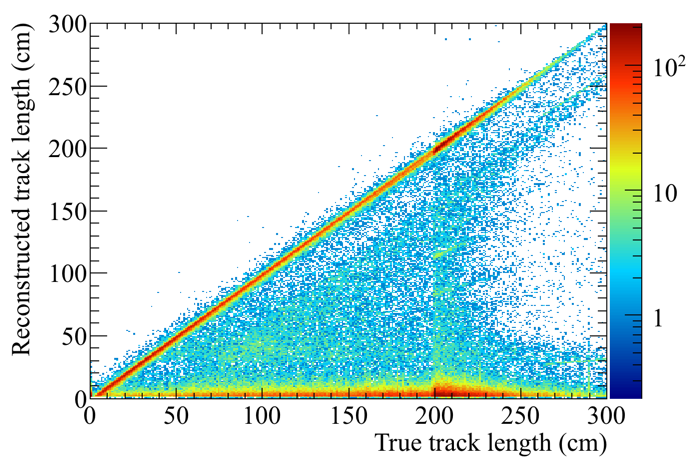
\includegraphics[width=\textwidth]{ProtonEnrich_500V_v05_14_00_trackpmtrackdc_Muon_All_MCRecoTrackLength}
        \caption{The relationship between reconstructed track length, and the track length from Monte Carlo truth, filled for all tracks.}
        \label{fig:CRY_MCRecoTrack_Muon_All}
  \end{subfigure}
  \caption[The calculated PIDA values, as a function of the reconstructed track length, for muons in the simulated proton enriched sample in the 35 ton detector]
          {The calculated PIDA values, as a function of the reconstructed track length, for muons in the simulated proton enriched sample in the 35 ton detector. Left: the PIDA values, as a function of the ratio between reconstructed track length, and the track length from Monte Carlo truth. Right, the relationship between reconstructed track length, and the track length from Monte Carlo truth. All plots are made for tracks which have been reconstructed using a cheated interaction time determination.}
  \label{fig:CRY_MuonAllComp}
\end{figure}

Figure~\ref{fig:CRY_PIDACuts}, shows the distribution of calculated PIDA values for protons and muons in the proton enriched CRY sample, after a cut on the minimum reconstructed track length of 10~cm is applied. \\

%%%%%%% The Normal PIDA plots after new cuts......
\begin{figure}
  \centering
  \begin{subfigure}{0.48\textwidth}
        \centering
        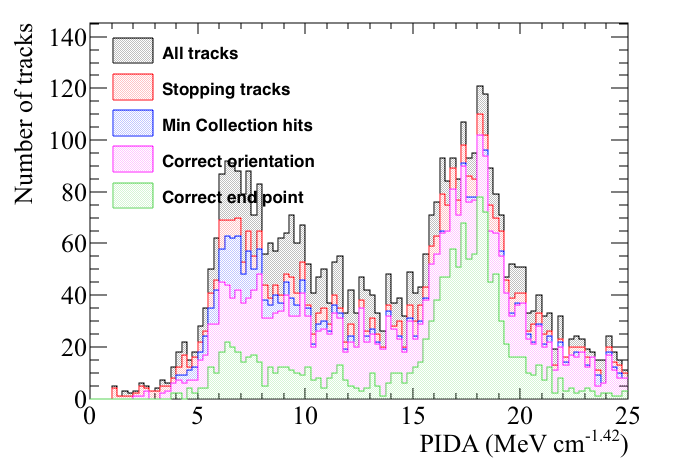
\includegraphics[width=\textwidth]{ProtonEnrich_500V_v05_14_00_trackpmtrackT0_MinTrCut_Proton_PIDA}
        \caption{The PIDA values calculated for protons, using the photon detectors to calculate an interaction time.}
        \label{fig:CRY_PIDACuts_Proton_NonCheat}
  \end{subfigure}%
  \hspace{0.03\textwidth}%
  \begin{subfigure}{0.48\textwidth}
        \centering
        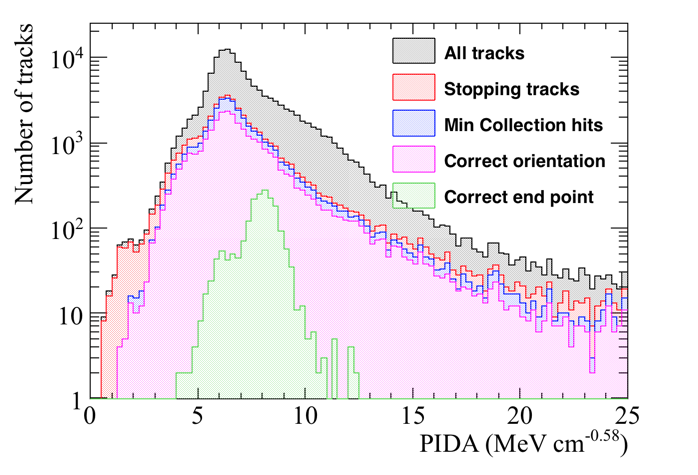
\includegraphics[width=\textwidth]{ProtonEnrich_500V_v05_14_00_trackpmtrackT0_MinTrCut_Muon_PIDA}
        \caption{The PIDA values calculated for muons, using the photon detectors to calculate an interaction time.}
        \label{fig:CRY_PIDACuts_Muon_NonCheat}
  \end{subfigure}
  %%%%%%%%%%%
  \begin{subfigure}{0.48\textwidth}
        \centering
        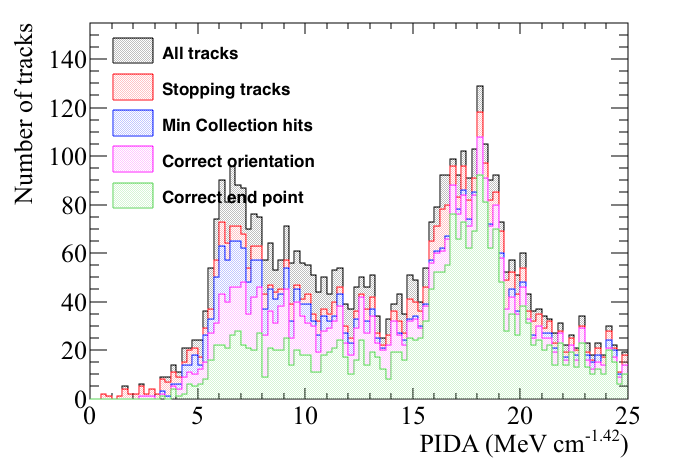
\includegraphics[width=\textwidth]{ProtonEnrich_500V_v05_14_00_trackpmtrackdc_MinTrCut_Proton_PIDA}
        \caption{The PIDA values calculated for protons, using a cheated interaction time determination.}
        \label{fig:CRY_PIDACuts_Proton_Cheat}
  \end{subfigure}%
  \hspace{0.03\textwidth}%
  \begin{subfigure}{0.48\textwidth}
        \centering
        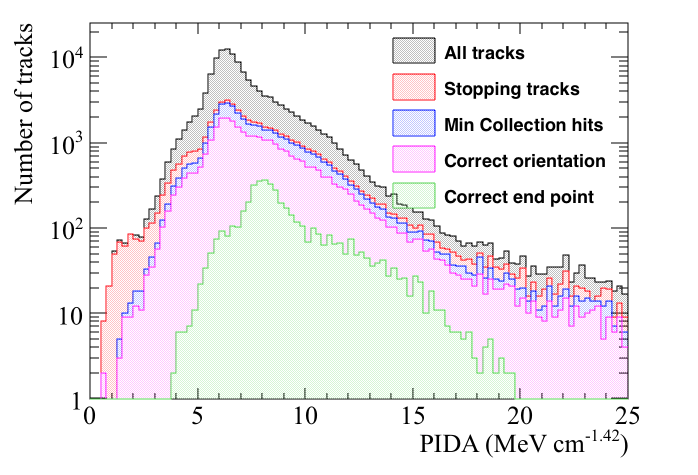
\includegraphics[width=\textwidth]{ProtonEnrich_500V_v05_14_00_trackpmtrackdc_MinTrCut_Muon_PIDA}
        \caption{The PIDA values calculated for muons, using a cheated interaction time determination.}
        \label{fig:CRY_PIDACuts_Muon_Cheat}
  \end{subfigure}
  \caption[The calculated PIDA values for the simulated proton enriched sample in the 35 ton detector, after a cut on the minimum reconstructed track length is applied]
          {The calculated PIDA values for the simulated proton enriched sample in the 35 ton detector, after a cut on the minimum reconstructed track length is applied. Top left: the PIDA values calculated for protons using the photon detectors to measure the interaction time. Top right: the PIDA values calculated for muons using the photon detectors to measure the interaction time. Bottom left: PIDA values calculated for protons using a cheated interaction time determination. Bottom right: the PIDA values calculated for muons using a cheated interaction time determination. The cut on minimum track length is applied before any graphs are filled. A series of criteria designed to select only tracks due to stopping particles which have a required number of collection plane hits is applied. The tracks are then further refined using truth information such as the true end point of the particle.}
  \label{fig:CRY_PIDACuts}
\end{figure}

When comparing Figures~\ref{fig:CRY_PIDA}, and~\ref{fig:CRY_PIDACuts}, the removal of muon tracks with PIDA values of 3 MeV$\cdot$cm$^{-1}$ is very apparent, and shows that the cut on the minimum reconstructed track length was successful. It can also be seen that the number of muon tracks which have PIDA values consistent with a proton has also decreased by around a factor of 2. However, this has come at the cost of some of the proton tracks which could have been correctly identified as protons being removed, due to their short track lengths. This is unfortunate, but some loss is unavoidable, as the significantly more numerous muons would overwhelm any proton tracks, should the identification be attempted in cosmic ray data collected by the 35~ton detector. The peak around PIDA values of 8 MeV$\cdot$cm$^{-1}$ for muon tracks, is however, only identifiable once the requirement that the end point of the reconstructed track is close to the end point of the particle from Monte Carlo truth. Therefore, a more robust system of cuts is required in order to produce a sample of muon tracks which can reliably identified as such. \\

As outlined above, partially reconstructed muon tracks have PIDA values of 6 MeV$\cdot$cm$^{-1}$, and so in order to remove the large peak of these tracks still seen in Figure~\ref{fig:CRY_PIDACuts}, some form of track stitching is required in order to remove these tracks. It is possible that a large number of these tracks are due to muons which pass through the detector, as many cosmic muons will do, but have been reconstructed as at least two separate tracks. Should this be the case, at least one of the tracks would be considered to ``stop'' in the detector. The effect of removing these split tracks can be seen in Figure~\ref{fig:CRY_PIDACheat}, where all particle which do not stop in the detector, from Monte Carlo truth, have been removed. This effectively ``cheats'' the stitching which is required to remove the majority of split muon tracks, though any muons which stop in the detector, but have been split into two or more tracks by the reconstruction, will still be present in Figure~\ref{fig:CRY_PIDACheat}. It can be seen that these tracks are still present, as there is still a peak in PIDA values of 6 MeV$\cdot$cm$^{-1}$, though these tracks are now overshadowed by tracks with PIDA values of 8 MeV$\cdot$cm$^{-1}$. \\

%%%%%%% The Cheated PIDA plots after new cuts......
\begin{figure}
  \centering
  \begin{subfigure}{0.48\textwidth}
        \centering
        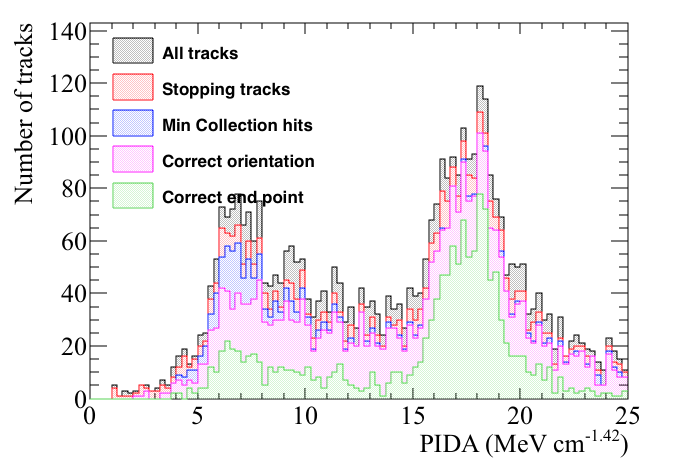
\includegraphics[width=\textwidth]{ProtonEnrich_500V_v05_14_00_trackpmtrackT0_MinTrCut_MCCont_Proton_PIDA}
        \caption{The PIDA values calculated for protons, using the photon detectors to calculate an interaction time.}
        \label{fig:CRY_PIDACheat_Proton_NonCheat}
  \end{subfigure}%
  \hspace{0.03\textwidth}%
  \begin{subfigure}{0.48\textwidth}
        \centering
        \includegraphics[width=\textwidth]{ProtonEnrich_500V_v05_14_00_trackpmtrackT0_MinTrCut_MCCont_Muon_PIDA}
        \caption{The PIDA values calculated for muons, using the photon detectors to calculate an interaction time.}
        \label{fig:CRY_PIDACheat_Muon_NonCheat}
  \end{subfigure}
  %%%%%%%%%%%
  \begin{subfigure}{0.48\textwidth}
        \centering
        \includegraphics[width=\textwidth]{ProtonEnrich_500V_v05_14_00_trackpmtrackdc_MinTrCut_MCCont_Proton_PIDA}
        \caption{The PIDA values calculated for protons, using a cheated interaction time determination.}
        \label{fig:CRY_PIDACheat_Proton_Cheat}
  \end{subfigure}%
  \hspace{0.03\textwidth}%
  \begin{subfigure}{0.48\textwidth}
        \centering
        \includegraphics[width=\textwidth]{ProtonEnrich_500V_v05_14_00_trackpmtrackdc_MinTrCut_MCCont_Muon_PIDA}
        \caption{The PIDA values calculated for muons, using a cheated interaction time determination.}
        \label{fig:CRY_PIDACheat_Muon_Cheat}
  \end{subfigure}
  \caption[The calculated PIDA values for the simulated proton enriched sample in the 35 ton detector, after tracks from particles which do not stop in the detector are removed]
          {The calculated PIDA values for the simulated proton enriched sample in the 35 ton detector, after tracks from particles which do not stop in the detector are removed. Top left: the PIDA values calculated for protons using the photon detectors to measure the interaction time. Top right: the PIDA values calculated for muons using the photon detectors to measure the interaction time. Bottom left: PIDA values calculated for protons using a cheated interaction time determination. Bottom right: the PIDA values calculated for muons using a cheated interaction time determination. The cut on minimum track length is applied before any graphs are filled, as is the cut on any reconstructed tracks which are associated with particles which do not stop in the detector, according to Monte Carlo truth. A series of criteria designed to select only tracks due to stopping particles which have a required number of collection plane hits is applied. The tracks are then further refined using truth information such as the true end point of the particle.}
  \label{fig:CRY_PIDACheat}
\end{figure}

The number of muon tracks with high PIDA values in all plots is concerning, though this is particularly true for those shown in Figure~\ref{fig:CRY_PIDACheat}, as these tracks are due to particles which stop in the detector, and are accurately reconstructed. This is because the contamination caused by these tracks, would mean that it would be difficult to ascertain whether a track with a PIDA value of around 18 is actually a proton. \\

The basic framework by which particle identification can occur has been outlined here, and is shown to be very effective when particles are simulated in isolation. It has also been shown that a clear separation between muons and protons can be seen in cosmic rays, though there is a non-negligible contamination of the proton track PIDA range by muon tracks. This separation was only possible when using information from Monte Carlo truth though, and so a more sophisticated method of identifying through-going muons is required, should the analysis be performed on the cosmic ray data, such as that collected by the 35 ton detector. \\
